%definira klasu dokumenta 
\documentclass[12pt]{report} 

%prostor izmedu naredbi \documentclass i \begin{document} se zove uvod. U njemu se nalaze naredbe koje se odnose na cijeli dokument

%osnovni LaTex ne može riješiti sve probleme, pa se koriste različiti paketi koji olakšavaju izradu željenog dokumenta
\usepackage[croatian]{babel} 
\usepackage{amssymb}
\usepackage{amsmath}
\usepackage{txfonts}
\usepackage{mathdots}
\usepackage{titlesec}
\usepackage{array}
\usepackage{lastpage}
\usepackage{etoolbox}
\usepackage{tabularray}
\usepackage{color, colortbl}
\usepackage{adjustbox}
\usepackage{geometry}
\usepackage[classicReIm]{kpfonts}
\usepackage[hidelinks]{hyperref}
\hypersetup{
	colorlinks   = true, %Colours links instead of ugly boxes
	urlcolor     = blue, %Colour for external hyperlinks
	linkcolor    = blue, %Colour of internal links
	citecolor   = red %Colour of citations
}
\usepackage{fancyhdr}

\usepackage{url} % Add this package to support URL formatting
\usepackage{graphicx}
\usepackage{helvet}

\usepackage{float}
\usepackage{setspace}
\restylefloat{table}


\patchcmd{\chapter}{\thispagestyle{plain}}{\thispagestyle{fancy}}{}{} %redefiniranje stila stranice u paketu fancyhdr

%oblik naslova poglavlja
\titleformat{\chapter}{\normalfont\huge\bfseries}{\thechapter.}{20pt}{\Huge}
\titlespacing{\chapter}{0pt}{0pt}{40pt}


\linespread{1.3} %razmak između redaka

\geometry{a4paper, left=1in, top=1in,}  %oblik stranice

\hypersetup{ colorlinks, citecolor=black, filecolor=black, linkcolor=black,	urlcolor=black }   %izgled poveznice


%prored smanjen između redaka u nabrajanjima i popisima
\newenvironment{packed_enum}{
	\begin{enumerate}
		\setlength{\itemsep}{0pt}
		\setlength{\parskip}{0pt}
		\setlength{\parsep}{0pt}
	}{\end{enumerate}}

\newenvironment{packed_item}{
	\begin{itemize}
		\setlength{\itemsep}{0pt}
		\setlength{\parskip}{0pt}
		\setlength{\parsep}{0pt}
	}{\end{itemize}}




%boja za privatni i udaljeni kljuc u tablicama
\definecolor{LightBlue}{rgb}{0.9,0.9,1}
\definecolor{LightGreen}{rgb}{0.9,1,0.9}

%Promjena teksta za dugačke tablice
\DefTblrTemplate{contfoot-text}{normal}{Nastavljeno na idućoj stranici}
\SetTblrTemplate{contfoot-text}{normal}
\DefTblrTemplate{conthead-text}{normal}{(Nastavljeno)}
\SetTblrTemplate{conthead-text}{normal}
\DefTblrTemplate{middlehead,lasthead}{normal}{Nastavljeno od prethodne stranice}
\SetTblrTemplate{middlehead,lasthead}{normal}

%podesavanje zaglavlja i podnožja

\pagestyle{fancy}
\lhead{Programsko inženjerstvo}
\rhead{SpotPicker}
\lfoot{Lukax4}
\cfoot{stranica \thepage/\pageref{LastPage}}
\rfoot{\today}
\renewcommand{\headrulewidth}{0.2pt}
\renewcommand{\footrulewidth}{0.2pt}


\begin{document} 
	
	
	
	    \begin{titlepage}
		\begin{center}
			\vspace*{\stretch{1.0}} %u kombinaciji s ostalim \vspace naredbama definira razmak između redaka teksta
			\LARGE Programsko inženjerstvo\\
			\large Ak. god. 2023./2024.\\
			
			\vspace*{\stretch{3.0}}
			
			\huge SpotPicker\\
			\Large Dokumentacija, Rev. \textit{1}\\
			
			\vspace*{\stretch{12.0}}
			\normalsize
			Grupa: \textit{Lukax4}\\
			Voditelj: \textit{Luka Diktić}\\
			
			
			\vspace*{\stretch{1.0}}
			Datum predaje: \textit{17. 11. 2023.}\\
			
			\vspace*{\stretch{4.0}}
			
			Nastavnik: \textit{Hrvoje Nuić, mag. ing.}\\
			
		\end{center}
		
		
	\end{titlepage}

	
	\tableofcontents


	\chapter{Dnevnik promjena dokumentacije}
		
		\textbf{\textit{}}\\
				
		
		\begin{longtblr}[
				label=none
			]{
				width = \textwidth, 
				colspec={|X[2]|X[13]|X[3]|X[3]|}, 
				rowhead = 1
			}
			\hline
			\textbf{Rev.}	& \textbf{Opis promjene/dodatka} & \textbf{Autori} & \textbf{Datum}\\[3pt] \hline
			0.1 & Napravljen predložak.	& Luka Žmak & 25.10.2023. 		\\[3pt] \hline 
			0.2	& Dopisane upute za povijest dokumentacije.\newline Dodane reference. & Maja Mavračić & 24.08.2013. 	\\[3pt] \hline 
			0.5 & Dodan \textit{Use Case} dijagram i jedan sekvencijski dijagram, funkcionalni i nefunkcionalni zahtjevi i dodatak A & Mirta Posnjak & 26.10.2023. \\[3pt] \hline 
			0.6 & Arhitektura i dizajn sustava, algoritmi i strukture podataka & Filip Sučić & 27.10.2013. \\[3pt] \hline 
			0.8 & Povijest rada i trenutni status implementacije,\newline Zaključci i plan daljnjeg rada & *Dominik Poljak & 2.11.2023. \\[3pt] \hline 
			0.9 & Opisi obrazaca uporabe & Luka Diktić & 07.11.2023. \\[3pt] \hline 
			0.10 & Preveden uvod & Luka Babić & 10.11.2023. \\[3pt] \hline 
			0.11 & Sekvencijski dijagrami & Mirta Posnjak & 15.11.2023. \\[3pt] \hline 
			0.12.2 & Napravljen dijagrama razreda & Maja Mavračić & 16.11.2023. \\[3pt] \hline 
			\textbf{1.0} & Verzija samo s bitnim dijelovima za 1. ciklus & svi & 17.11.2023. \\[3pt] \hline 
			1.1 & Implementacija	& Luka Žmak & 25.11.2023. \\[3pt] \hline 
			1.2& Dodani dijagram stanja i dijagram aktivnosti 	& Luka Diktić & 25.11.2023. \\[3pt] \hline 
			1.3 & Dodan dijagram razmjestaja 	& Maja Mavračić & 5.1.2024. \\[3pt] \hline 
			1.4 & Dodan opis tehnologija i alata 	& Mirta Posnjak & 5.1.2024. \\[3pt] \hline 
			1.5 & Dodan dio korisnickih uputa	& Dominik Poljak & 10.1.2024. \\[3pt] \hline 
			1.6 & Dodan dijagram komponenti 	& Filip Sučić & 15.1.2024. \\[3pt] \hline 
			1.7 & Konacne korisničke upute	& Luka Babić & 15.1.2024. \\[3pt] \hline 
			1.8 & Dodana potrebna instalacija 	& Luka Žmak & 17.1.2024. \\[3pt] \hline 
			1.9 & Pregledano i dodane slike s opisima	& Luka Diktić & 17.1.2024. \\[3pt] \hline 
			2.0 & Konacna verzija 	&  &  \\[3pt] \hline 
		
		\end{longtblr}
	
	
		\textit{}
		 \section{Opis projektnog zadatka}
	
	
	
	\hspace{1cm}{\Large Cilj projekta je napraviti web aplikaciju “SpotPicker” koja bi omogućila vozačima osobnih automobile i bicikla da unaprijed rezerviraju svoje parkirno mjeto u garaži i time se riješe svakodnevne muke lutanja po parkingu i traženja mjesta.\\}
	
	\hspace{1cm}{\Large S korisničke strane, aplikacija se otvara u neregistriranom obliku. Neregistrirani korisnik moze pregledavati parkirališta i njihova parkirna mjesta, ali bez informacije o dostupnosti. Zato se novim korisnicima nudi mogućnost registracije, odnosno izrade korisničkog računa i mogućnost prijave za one koji već imaju izrađen račun. Za registraciju su potrebni:}
	\begin{itemize}
		\item \textit{{\Large korisničko ime}}
		\item \textit{{\Large lozinka}}
		\item \textit{{\Large ime}}
		\item \textit{{\Large prezime}}
		\item \textit{{\Large slika osobne}}
		\item \textit{{\Large IBAN račun}}
		\item \textit{{\Large email adresa\\}}
	\end{itemize} 
	
	 \hspace{1cm}{\Large 	Prilikom prve registracije potrebno je potvrditi svoje podatke preko poruke poslane na prethodno unesenu e-mail adresu. Za prijavu su potrebni samo korisničko ime i lozinka. Najvažnija dodatna mogućnost koju aplikacija nudi prijavljenim korisnicima je pregled dostupnih parkirnih mjesta u realnom vremenu. Puni postupak rezervacije parkirnog mjesta izgleda ovako:}
	\begin{itemize}
		\item[] {\Large 1. korisnik na karti grada bira lokaciju do koje želi doći}
		\item[] {\Large 2. aplikacija mu na temelju njegovog odredišta bira najbliži parking}
	\end{itemize}
	{\Large Sljedeći se korak može odviti na dva načina:}
	\begin{itemize}
		\item[] {\Large 3. a) korisnik bira parkirna mjesta koja mu se sviđaju, a zatim se otvara kalendar u kojem može točno odabrati termin rezervacije (datum i vrijeme)}
		\item[] {\Large 3. b) korisnik bira termin rezervacije (datum i vrijeme), a zatim mu se prikazuju parkirna mjesta koja će tada biti dostupna}
	\end{itemize}
	{\Large Ovdje je bitno napomenuti da i u a) i u b) varijanti najranija moguća rezervacija je dan nakon onog u kojem korisnik vrši rezervaciju. Znači nije moguće rezervirati na isti dan.}
	\begin{itemize}
		\item[] {\Large 4. korisnik sada dobiva dodatnu mogućnost odabira želi li da mu rezervacija bude ponavljajuća ili ne. To je pogotovo pogodno ljudima koji znaju da imaju neke obaveze na npr. tjednoj bazi}
		\item[] {\Large 5. korisniku se daje opcija plaćanja karticom unaprijed ili plaćanje prilikom dolaska na parking}
		\item[] {\Large 6. potvrđuje se rezervacija parkirnog mjesta, termina, trajanja i načina plaćanja\\ \\ }
	\end{itemize}
	

	\hspace{1cm}{\Large Korisniku se pruža mogućnost plaćanja direktnim prijenosom sredstava s kartice ili uplaćivanjem novca u novčanik unutar aplikacije nakon kojeg se sredstva mogu koristiti u bilo kojem trenutku. Drugi način štedi vrijeme jer nije potrebno unositi podatke o kartici i vršiti potvrde prilikom svake transakcije.\\ }
	
	\hspace{1cm}{\Large Šta se tiče parkirnih mjesta za bicikle, njih nije potrebno rezervirati jer se ne naplaćuju. Moguće je jedino pratiti u realnom vremenu ukupan broj dostupnih mjesta.\\}
	
	\hspace{1cm}{\Large }
	
	\hspace{1cm}{\Large U slučaju da se korisnik prijavljuje kao voditelj parkinga, da bi dobio voditeljska prava prvo je potrebno odobrenje administratora. Voditelj ima mogućnost promjene podataka o svom parking. To uključuje izmjenu imena parkinga, dodavanje i uklanjanje slika te promjene cijena. Također može dodavati nova mjesta u slučaju proširenja parkinga.\\}
	
	\hspace{1cm}{\Large Uloga administratora donosi pravo pregledavanja i mijenjanja osobnih podataka registriranih korisnika. Također, on potvrđuje identitet voditelja parking prilikom prijave u aplikaciju. \\}
	
	\hspace{1cm}{\Large Slično programsko rješenje nudi aplikacija JustPark koja omogućuje rezervaciju parkirnih mjesta u Ujedinjenom Kraljevstvu. Glavno sučelje \hyperref[fig:justpark1]{(slika1)} nudi jednastavnu mogućnost odabira lokacije i termina. Zatim se otvara popis parkirališta sortiranih po  udaljenosti koju treba pješice prijeći od parking do finalne destinacije. SpotPicker se razlikuje od JustParka po tome šta JustPark nudi ostavljanje komentara i ocijenjivanje parkinga \hyperref[fig:justpark2]{(slika2)} po raznim kriterijima poput sigurnosti, lakoće snalaženja, širine mjesta itd.\\}
	
	\clearpage
	
	% Unos slike
	\begin{figure}[]
		\centering
		\fbox{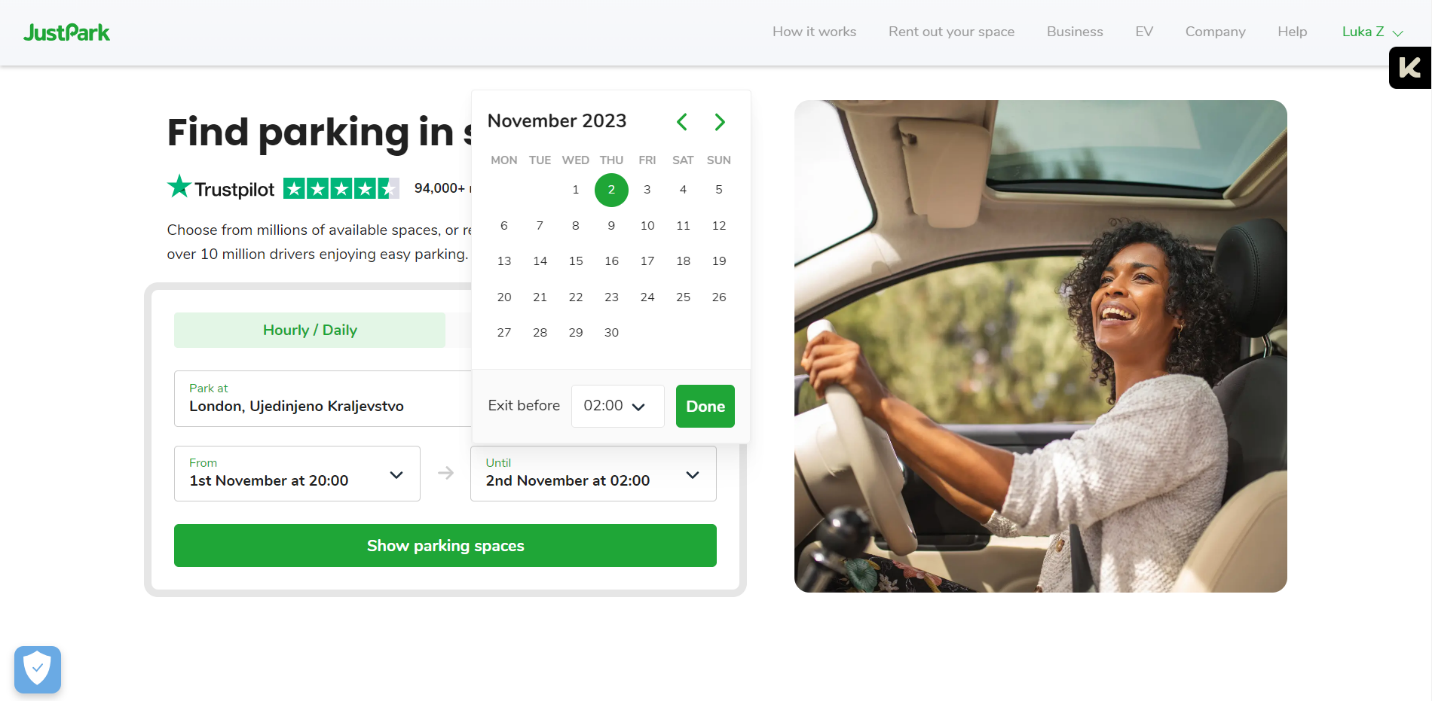
\includegraphics[]{slike/justPark1.png}}
		\caption{Sučelje za odabir termina u JustPark}
		\label{fig:justpark1}
	\end{figure}
	
	\begin{figure}[!ht]
		\centering
		\fbox{\includegraphics[]{slike/justPark2.png}}
		\caption{Dodatna mogućnost ocjene parkinga u JustPark}
		\label{fig:justpark2}
	\end{figure}
	
	\clearpage
	
	\hspace{1cm}{\Large SpotPicker je aplikacija savršena za ljude koji planiraju svoja putovanja ili obaveze po nekoliko dana unaprijed jer će si rezervacijom mjesta ukloniti onaj najgori dio vožnje, a to je lutanje u potrazi za mjestom. Također, pogodno je ljudima koji moraju negdje doći na vrijeme jer ovako mogu značajno bolje procijeniti koliko im je vremena potrebno u vožnji. Isto tako, aplikaciju mogu korisiti i ljudi kojima je parking potreban stalno (npr. jer rade u blizini) jer je moguće da rezervacija bude ponavljajuća iz tjedna u tjedan.\\}
	
	\hspace{1cm}{\Large Naravno, bitno je napomenuti da je ovaj project moguće nadograditi i poboljšati neke njegove stavke. Tako bi korisni dodatak bio mogućnost poništavanja rezervacije uz povrat novca.\\}
	
	\hspace{1cm}{\Large Šta se tiče prilagodbe raznim tržištima, za manje gradove koji imaju puno privatnih kuća u centru, bila bi dobra mogućnost da se vlasnici kuća s dvorištem mogu prijaviti da iznajmljuju svoje dvorište kao parkirno mjesto. Vlasnik dvorišta bi se jednako vodio kao i vlasnik većeg parkirališta, a odabir mjesta bi djelovao na isti način kao i kod velikih parkinga ovisno o veličini dvorišta. Bitno je primijetiti da projekt uključuje rješenje za parkirališta s jednom razinom, tako da bi jedno dodatno moguće proširenje bilo dodati mogućnost odabira kata garaže i tek onda parkirnog mjesta. \\}
	

	


	\chapter{Specifikacija programske potpore}
		
	\section{Funkcionalni zahtjevi}
			
			
			\noindent \textbf{Dionici:}
			
			
			\begin{packed_enum}
				
				\item Korisnik
				\item Administrator				
				\item Vlasnik parkirališta(naručitelj)
				\item Razvojni tim
				
			\end{packed_enum}
			
			\noindent \textbf{Aktori i njihovi funkcionalni zahtjevi:}
			
			
			\begin{packed_enum}
				\item  \underbar{Neregistrirani korisnik (inicijator) može:}
				
				\begin{packed_enum}
					\item na karti pregledati lokacije parkirališta i tlocrt parkirališta
					\item stvoriti korisnički račun, tj. registrirati se za šta su mu potrebni korisničko ime, lozinka,  ime, prezime, slika osobne iskaznice, IBAN i email adresa 
				\end{packed_enum}
			
				\item  \underbar{Registrirani korisnik (sudionik) može:}
				
				\begin{packed_enum}
					\item prijaviti se u sustav koristeći korisničko ime i lozinku
					\item na karti odabrati adresu do koje želi doći
					\item na karti pregledati lokacije parkirališta, tlocrt parkirališta i dostupna parkirna mjesta
					\item rezervirati parkirno mjesto, termin i trajanje za koje je zainteresiran
					\item platiti rezervaciju parkinga 
				\end{packed_enum}
				
				\item  \underbar{Vlasnik parkinga (sudionik) može:}
				
				\begin{packed_enum}
					\item unijeti i mijenjati informacije o svom parkiralištu (naziv, opis, fotografija, cjenik)
					\item dodavati nova parkirna mjesta
					\item vidjeti statistiku zauzetosti parkirališta i parkirališnih mjesta kroz vrijeme
			 	\end{packed_enum}
			 	
				\item  \underbar{Administrator (sudionik) može:}
				
				\begin{packed_enum}
					\item pregledavati osobne podatke registriranih korisnika
					\item mijenjati osobne podatke registriranih korisnika
					\item potvrditi prijavu korisnicima koji se prijavljuju kao vlasnik parkinga
					
				\end{packed_enum}
			\end{packed_enum}
			\eject 
			
			
				
			\subsection{Obrasci uporabe}
				
				\subsubsection{Opis obrazaca uporabe}
					
					\noindent \underbar{\textbf{UC1 - registracija korisnika}}
					\begin{packed_item}
						
						\item \textbf{Glavni sudionik: }neregistrirani korisnik
						\item  \textbf{Cilj:} izraditi korisnički račun
						\item  \textbf{Sudionici:} baza podataka
						\item  \textbf{Preduvjet:} -
						\item  \textbf{Opis osnovnog tijeka:}
						
						\item[] \begin{packed_enum}
							
							\item korisnik odabire opciju za registraciju
							\item korisnik upisuje potrebne podatke
							\item u bazu podataka se upisuje novi korisnik
							\item web stranica se preusmjerava na stranicu za prijavu 
					
						\end{packed_enum}
						
						\item  \textbf{Opis mogućih odstupanja:}
						
						\item[] \begin{packed_item}
							
							\item[2.a] korisničko ime i/ili email su već zauzeti
							\item[] \begin{packed_enum}
								
								\item korisnik dobiva povratnu informaciju o specifičnoj greški i preusmjeren je nazad na stranicu za              registraciju
								
								
							\end{packed_enum}
							\item[2.b] upisana lozinka nije važeća(nema barem 8 znakova ili ne sadrži barem jedno slovo i brojku)
							\begin{packed_enum}
								
								\item korisnik dobiva povratnu informaciju o specifičnoj greški i preusmjeren je nazad na stranicu za              registraciju
								
								
							\end{packed_enum}
							
						\end{packed_item}
					\end{packed_item}
					
					\noindent \underbar{\textbf{UC2 -prijava korisnika}}
					\begin{packed_item}
						
						\item \textbf{Glavni sudionik: }registrirani korisnik
						\item  \textbf{Cilj:} prijava u korisnički račun
						\item  \textbf{Sudionici:} baza podataka
						\item  \textbf{Preduvjet:} prethodna registracija
						\item  \textbf{Opis osnovnog tijeka:}
						
						\item[] \begin{packed_enum}
							
							\item korisnik odabire opciju za prijavu
							\item korisnik upisuje svoje korisničko ime i lozinku
							\item korisnik je preusmjeren na početnu stranicu sa svim ovlastima prijavljenog korisnika
						
						\end{packed_enum}
						
						\item  \textbf{Opis mogućih odstupanja:}
						
						\item[] \begin{packed_item}
							
							\item[2.a] upisana kombinacija korisničkog imena i lozinke je neispravna
							\item[] \begin{packed_enum}
								
								\item korisnik je vraćen na stranicu za prijavu
								
							\end{packed_enum}
						
							
						\end{packed_item}
					\end{packed_item}
					
					\noindent \underbar{\textbf{UC3-promjena lozinke}}
					\begin{packed_item}
	
						\item \textbf{Glavni sudionik: }registrirani korisnik
						\item  \textbf{Cilj:} izmijeniti lozinku na već postojećem korisničkom računu
						\item  \textbf{Sudionici:} baza podataka
						\item  \textbf{Preduvjet:} prethodna registracija
						\item  \textbf{Opis osnovnog tijeka:}
						
						\item[] \begin{packed_enum}
	
							\item korisnik izabire opciju za mijenjanje lozinku
							\item korisnik upisuje email adresu na koju želi da mu se pošalje verifikacijski kod
							\item korisnik upisuje verifikacijski kod
							\item korisnik upisuje novu lozinku i potvrđuje ju ponovnim upisom
							\item korisnik je preusmjeren na stranicu za prijavu
						\end{packed_enum}
						
						\item  \textbf{Opis mogućih odstupanja:}
						
						\item[] \begin{packed_item}
	
							\item[3.a] upisani verifikacijski kod nije isti onom poslanom na email
							\item[] \begin{packed_enum}
								
								\item dolazi poruka o grešci i korisnik može opet upisati kod
								
							\end{packed_enum}
							\item[4.a] lozinke se ne poklapaju
							
							\begin{packed_enum}
								
								\item dolazi poruka o grešci i korisnik može opet upisati loznike
								
							\end{packed_enum}
							
							\item[4.b] upisana lozinka nije važeća(nema barem 8 znakova ili ne sadrži barem jedno slovo i brojku)
							
							\begin{packed_enum}
								
								\item dolazi poruka o grešci i korisnik može opet upisati loznike
								
							\end{packed_enum}
							
						\end{packed_item}
					\end{packed_item}
					
					\noindent \underbar{\textbf{UC4-odabir parkirališta}}
					\begin{packed_item}
						
						\item \textbf{Glavni sudionik: }prijavljeni korisnik
						\item  \textbf{Cilj:} izabrati parkiralište na kojem će kasnije rezervirati mjesto
						\item  \textbf{Sudionici:} sudionici
						\item  \textbf{Preduvjet:} prethodna prijava
						\item  \textbf{Opis osnovnog tijeka:}
						
						\item[] \begin{packed_enum}
							
							\item korisnik upisuje adresu do koje želi doći
							\item korisnik kliklne gumb za pretraživanje
							\item korisniku se na karti iscrta ruta do parkirališta koje je najbliže njegovom odredištu
						
						\end{packed_enum}
						
						 
					\end{packed_item}
					
					\noindent \underbar{\textbf{UC5.1 -rezervacija mjesta s uvjetom određenog mjesta}}
					\begin{packed_item}
						
						\item \textbf{Glavni sudionik: }prijavljeni korisnik
						\item  \textbf{Cilj:} rezervirati specifično parkirno mjesto
						\item  \textbf{Sudionici:} sudionici
						\item  \textbf{Preduvjet:} odabrano parkiralište
						\item  \textbf{Opis osnovnog tijeka:}
						
						\item[] \begin{packed_enum}
							
							\item korisnik klikne na ikonu parkirališta
							\item na karti parkirališta odabire mjesto za koje je zainteresiran
							\item u kalendaru izabire datum
							\item korisniku se prikazuju slobodni sati za odabrano mjesto i datum
							\item korisnik bira vremensko razdoblje
							\item korisnik potvrđuje rezervaciju
							\item web stranica se preusmjerava na stranicu za plaćanje
						\end{packed_enum}
						
						\item  \textbf{Opis mogućih odstupanja:}
						
						\item[] \begin{packed_item}
							
							\item[4.a] sva vremena za taj datum i mjesto su zauzeti
							\item[] \begin{packed_enum}
								
								\item korisnik sam mora odabrati neki drugi datum ili mjesto
								
							\end{packed_enum}
							
						\end{packed_item}
					\end{packed_item}
					
					\noindent \underbar{\textbf{UC5.2-rezervacija mjesta s uvjetom datuma}}
					\begin{packed_item}
						
						\item \textbf{Glavni sudionik: }prijavljeni korisnik
						\item  \textbf{Cilj:} rezervirati mjesto u specifičnom terminu
						\item  \textbf{Sudionici:} sudionici
						\item  \textbf{Preduvjet:} odabrano parkiralište
						\item  \textbf{Opis osnovnog tijeka:}
						
						\item[] \begin{packed_enum}
							
							\item korisnik klikne na ikonu parkirališta
							\item korisnik u kalendaru odabire datum i vrijeme početka parkiranja
							\item korisnik u kalendaru odabire datum i vrijeme završetka parkiranja 
							\item korisniku se prikažu dostupna mjesta za odabrani termin na karti parkirališta
							\item korisnik odabire mjesto na karti
							\item korisnik potvrđuje rezervaciju
							\item web stranica se preusmjerava na stranicu za plaćanje
						\end{packed_enum}
						
						\item  \textbf{Opis mogućih odstupanja:}
						
						\item[] \begin{packed_item}
							
							\item[4.a]niti jedno mjesto se ne prikazuje kao dostupno
							\item[] \begin{packed_enum}
								
								\item korisnik mora odabrati drugi termin
								
								
							\end{packed_enum}
							
							
						\end{packed_item}
					\end{packed_item}
					
					\noindent \underbar{\textbf{UC6.1-plaćanje prilikom dolaska}}
					\begin{packed_item}
						
						\item \textbf{Glavni sudionik: }prijavljeni korisnik
						\item  \textbf{Cilj:} cilj
						\item  \textbf{Sudionici:} sudionici
						\item  \textbf{Preduvjet:} preduvjet
						\item  \textbf{Opis osnovnog tijeka:}
						
						\item[] \begin{packed_enum}
							
							\item opis korak jedan
							\item opis korak dva
							\item opis korak tri
							\item opis korak četiri
							\item opis korak pet
						\end{packed_enum}
						
						\item  \textbf{Opis mogućih odstupanja:}
						
						\item[] \begin{packed_item}
							
							\item[2.a] opis mogućeg scenarija odstupanja u koraku 2
							\item[] \begin{packed_enum}
								
								\item opis rješenja mogućeg scenarija korak 1
								\item opis rješenja mogućeg scenarija korak 2
								
							\end{packed_enum}
							\item[2.b] opis mogućeg scenarija odstupanja u koraku 2
							\item[3.a] opis mogućeg scenarija odstupanja  u koraku 3
							
						\end{packed_item}
					\end{packed_item}
					
					\noindent \underbar{\textbf{UC6.2-plaćanje karticom}}
					\begin{packed_item}
						
						\item \textbf{Glavni sudionik: }prijavljeni korisnik
						\item  \textbf{Cilj:} cilj
						\item  \textbf{Sudionici:} sudionici
						\item  \textbf{Preduvjet:} preduvjet
						\item  \textbf{Opis osnovnog tijeka:}
						
						\item[] \begin{packed_enum}
							
							\item opis korak jedan
							\item opis korak dva
							\item opis korak tri
							\item opis korak četiri
							\item opis korak pet
						\end{packed_enum}
						
						\item  \textbf{Opis mogućih odstupanja:}
						
						\item[] \begin{packed_item}
							
							\item[2.a] opis mogućeg scenarija odstupanja u koraku 2
							\item[] \begin{packed_enum}
								
								\item opis rješenja mogućeg scenarija korak 1
								\item opis rješenja mogućeg scenarija korak 2
								
							\end{packed_enum}
							\item[2.b] opis mogućeg scenarija odstupanja u koraku 2
							\item[3.a] opis mogućeg scenarija odstupanja  u koraku 3
							
						\end{packed_item}
					\end{packed_item}
					
					\noindent \underbar{\textbf{UC6.3-plaćanje sredstvima u novčaniku aplikacije}}
					\begin{packed_item}
						
						\item \textbf{Glavni sudionik: }prijavljeni korisnik
						\item  \textbf{Cilj:} cilj
						\item  \textbf{Sudionici:} sudionici
						\item  \textbf{Preduvjet:} preduvjet
						\item  \textbf{Opis osnovnog tijeka:}
						
						\item[] \begin{packed_enum}
							
							\item opis korak jedan
							\item opis korak dva
							\item opis korak tri
							\item opis korak četiri
							\item opis korak pet
						\end{packed_enum}
						
						\item  \textbf{Opis mogućih odstupanja:}
						
						\item[] \begin{packed_item}
							
							\item[2.a] opis mogućeg scenarija odstupanja u koraku 2
							\item[] \begin{packed_enum}
								
								\item opis rješenja mogućeg scenarija korak 1
								\item opis rješenja mogućeg scenarija korak 2
								
							\end{packed_enum}
							\item[2.b] opis mogućeg scenarija odstupanja u koraku 2
							\item[3.a] opis mogućeg scenarija odstupanja  u koraku 3
							
						\end{packed_item}
					\end{packed_item}
					
					\noindent \underbar{\textbf{UC7-dodavanje novaca u novčanik aplikacije}}
					\begin{packed_item}
						
						\item \textbf{Glavni sudionik: }prijavljeni korisnik
						\item  \textbf{Cilj:} cilj
						\item  \textbf{Sudionici:} sudionici
						\item  \textbf{Preduvjet:} preduvjet
						\item  \textbf{Opis osnovnog tijeka:}
						
						\item[] \begin{packed_enum}
							
							\item opis korak jedan
							\item opis korak dva
							\item opis korak tri
							\item opis korak četiri
							\item opis korak pet
						\end{packed_enum}
						
						\item  \textbf{Opis mogućih odstupanja:}
						
						\item[] \begin{packed_item}
							
							\item[2.a] opis mogućeg scenarija odstupanja u koraku 2
							\item[] \begin{packed_enum}
								
								\item opis rješenja mogućeg scenarija korak 1
								\item opis rješenja mogućeg scenarija korak 2
								
							\end{packed_enum}
							\item[2.b] opis mogućeg scenarija odstupanja u koraku 2
							\item[3.a] opis mogućeg scenarija odstupanja  u koraku 3
							
						\end{packed_item}
					\end{packed_item}
					
					\noindent \underbar{\textbf{UC8-izmjena osobnih podataka korisnika}}
					\begin{packed_item}
						
						\item \textbf{Glavni sudionik: }administrator
						\item  \textbf{Cilj:} cilj
						\item  \textbf{Sudionici:} sudionici
						\item  \textbf{Preduvjet:} preduvjet
						\item  \textbf{Opis osnovnog tijeka:}
						
						\item[] \begin{packed_enum}
							
							\item opis korak jedan
							\item opis korak dva
							\item opis korak tri
							\item opis korak četiri
							\item opis korak pet
						\end{packed_enum}
						
						\item  \textbf{Opis mogućih odstupanja:}
						
						\item[] \begin{packed_item}
							
							\item[2.a] opis mogućeg scenarija odstupanja u koraku 2
							\item[] \begin{packed_enum}
								
								\item opis rješenja mogućeg scenarija korak 1
								\item opis rješenja mogućeg scenarija korak 2
								
							\end{packed_enum}
							\item[2.b] opis mogućeg scenarija odstupanja u koraku 2
							\item[3.a] opis mogućeg scenarija odstupanja  u koraku 3
							
						\end{packed_item}
					\end{packed_item}
					
					\noindent \underbar{\textbf{UC9-potvrđivanje prijave vlasniku}}
					\begin{packed_item}
						
						\item \textbf{Glavni sudionik: }administrator
						\item  \textbf{Cilj:} cilj
						\item  \textbf{Sudionici:} sudionici
						\item  \textbf{Preduvjet:} preduvjet
						\item  \textbf{Opis osnovnog tijeka:}
						
						\item[] \begin{packed_enum}
							
							\item opis korak jedan
							\item opis korak dva
							\item opis korak tri
							\item opis korak četiri
							\item opis korak pet
						\end{packed_enum}
						
						\item  \textbf{Opis mogućih odstupanja:}
						
						\item[] \begin{packed_item}
							
							\item[2.a] opis mogućeg scenarija odstupanja u koraku 2
							\item[] \begin{packed_enum}
								
								\item opis rješenja mogućeg scenarija korak 1
								\item opis rješenja mogućeg scenarija korak 2
								
							\end{packed_enum}
							\item[2.b] opis mogućeg scenarija odstupanja u koraku 2
							\item[3.a] opis mogućeg scenarija odstupanja  u koraku 3
							
						\end{packed_item}
					\end{packed_item}
					
					\noindent \underbar{\textbf{UC10-brisanje korisnika}}
					\begin{packed_item}
						
						\item \textbf{Glavni sudionik: }administrator
						\item  \textbf{Cilj:} cilj
						\item  \textbf{Sudionici:} sudionici
						\item  \textbf{Preduvjet:} preduvjet
						\item  \textbf{Opis osnovnog tijeka:}
						
						\item[] \begin{packed_enum}
							
							\item opis korak jedan
							\item opis korak dva
							\item opis korak tri
							\item opis korak četiri
							\item opis korak pet
						\end{packed_enum}
						
						\item  \textbf{Opis mogućih odstupanja:}
						
						\item[] \begin{packed_item}
							
							\item[2.a] opis mogućeg scenarija odstupanja u koraku 2
							\item[] \begin{packed_enum}
								
								\item opis rješenja mogućeg scenarija korak 1
								\item opis rješenja mogućeg scenarija korak 2
								
							\end{packed_enum}
							\item[2.b] opis mogućeg scenarija odstupanja u koraku 2
							\item[3.a] opis mogućeg scenarija odstupanja  u koraku 3
							
						\end{packed_item}
					\end{packed_item}
					
					\noindent \underbar{\textbf{UC11-unos podataka o parkiralištu}}
					\begin{packed_item}
						
						\item \textbf{Glavni sudionik: }vlasnik
						\item  \textbf{Cilj:} cilj
						\item  \textbf{Sudionici:} sudionici
						\item  \textbf{Preduvjet:} preduvjet
						\item  \textbf{Opis osnovnog tijeka:}
						
						\item[] \begin{packed_enum}
							
							\item opis korak jedan
							\item opis korak dva
							\item opis korak tri
							\item opis korak četiri
							\item opis korak pet
						\end{packed_enum}
						
						\item  \textbf{Opis mogućih odstupanja:}
						
						\item[] \begin{packed_item}
							
							\item[2.a] opis mogućeg scenarija odstupanja u koraku 2
							\item[] \begin{packed_enum}
								
								\item opis rješenja mogućeg scenarija korak 1
								\item opis rješenja mogućeg scenarija korak 2
								
							\end{packed_enum}
							\item[2.b] opis mogućeg scenarija odstupanja u koraku 2
							\item[3.a] opis mogućeg scenarija odstupanja  u koraku 3
							
						\end{packed_item}
					\end{packed_item}
					
					\noindent \underbar{\textbf{UC12-dodavanje dostupnosti parkirnog mjesta}}
					\begin{packed_item}
						
						\item \textbf{Glavni sudionik: }vlasnik
						\item  \textbf{Cilj:} cilj
						\item  \textbf{Sudionici:} sudionici
						\item  \textbf{Preduvjet:} preduvjet
						\item  \textbf{Opis osnovnog tijeka:}
						
						\item[] \begin{packed_enum}
							
							\item opis korak jedan
							\item opis korak dva
							\item opis korak tri
							\item opis korak četiri
							\item opis korak pet
						\end{packed_enum}
						
						\item  \textbf{Opis mogućih odstupanja:}
						
						\item[] \begin{packed_item}
							
							\item[2.a] opis mogućeg scenarija odstupanja u koraku 2
							\item[] \begin{packed_enum}
								
								\item opis rješenja mogućeg scenarija korak 1
								\item opis rješenja mogućeg scenarija korak 2
								
							\end{packed_enum}
							\item[2.b] opis mogućeg scenarija odstupanja u koraku 2
							\item[3.a] opis mogućeg scenarija odstupanja  u koraku 3
							
						\end{packed_item}
					\end{packed_item}
					
					\noindent \underbar{\textbf{UC13-micanje dostupnosti parkirnog mjesta}}
					\begin{packed_item}
						
						\item \textbf{Glavni sudionik: }vlasnik
						\item  \textbf{Cilj:} cilj
						\item  \textbf{Sudionici:} sudionici
						\item  \textbf{Preduvjet:} preduvjet
						\item  \textbf{Opis osnovnog tijeka:}
						
						\item[] \begin{packed_enum}
							
							\item opis korak jedan
							\item opis korak dva
							\item opis korak tri
							\item opis korak četiri
							\item opis korak pet
						\end{packed_enum}
						
						\item  \textbf{Opis mogućih odstupanja:}
						
						\item[] \begin{packed_item}
							
							\item[2.a] opis mogućeg scenarija odstupanja u koraku 2
							\item[] \begin{packed_enum}
								
								\item opis rješenja mogućeg scenarija korak 1
								\item opis rješenja mogućeg scenarija korak 2
								
							\end{packed_enum}
							\item[2.b] opis mogućeg scenarija odstupanja u koraku 2
							\item[3.a] opis mogućeg scenarija odstupanja  u koraku 3
							
						\end{packed_item}
					\end{packed_item}
					
					\noindent \underbar{\textbf{UC14-pregledavanje statistike za parkiralište}}
					\begin{packed_item}
						
						\item \textbf{Glavni sudionik: }vlasnik
						\item  \textbf{Cilj:} cilj
						\item  \textbf{Sudionici:} sudionici
						\item  \textbf{Preduvjet:} preduvjet
						\item  \textbf{Opis osnovnog tijeka:}
						
						\item[] \begin{packed_enum}
							
							\item opis korak jedan
							\item opis korak dva
							\item opis korak tri
							\item opis korak četiri
							\item opis korak pet
						\end{packed_enum}
						
						\item  \textbf{Opis mogućih odstupanja:}
						
						\item[] \begin{packed_item}
							
							\item[2.a] opis mogućeg scenarija odstupanja u koraku 2
							\item[] \begin{packed_enum}
								
								\item opis rješenja mogućeg scenarija korak 1
								\item opis rješenja mogućeg scenarija korak 2
								
							\end{packed_enum}
							\item[2.b] opis mogućeg scenarija odstupanja u koraku 2
							\item[3.a] opis mogućeg scenarija odstupanja  u koraku 3
							
						\end{packed_item}
					\end{packed_item}
					
					\noindent \underbar{\textbf{UCbroj obrasca -ime obrasca}}
					\begin{packed_item}
						
						\item \textbf{Glavni sudionik: }sudionik
						\item  \textbf{Cilj:} cilj
						\item  \textbf{Sudionici:} sudionici
						\item  \textbf{Preduvjet:} preduvjet
						\item  \textbf{Opis osnovnog tijeka:}
						
						\item[] \begin{packed_enum}
							
							\item opis korak jedan
							\item opis korak dva
							\item opis korak tri
							\item opis korak četiri
							\item opis korak pet
						\end{packed_enum}
						
						\item  \textbf{Opis mogućih odstupanja:}
						
						\item[] \begin{packed_item}
							
							\item[2.a] opis mogućeg scenarija odstupanja u koraku 2
							\item[] \begin{packed_enum}
								
								\item opis rješenja mogućeg scenarija korak 1
								\item opis rješenja mogućeg scenarija korak 2
								
							\end{packed_enum}
							\item[2.b] opis mogućeg scenarija odstupanja u koraku 2
							\item[3.a] opis mogućeg scenarija odstupanja  u koraku 3
							
						\end{packed_item}
					\end{packed_item}
				
					
				\subsubsection{Dijagrami obrazaca uporabe}
					
					\textit{Prikazati odnos aktora i obrazaca uporabe odgovarajućim UML dijagramom. Nije nužno nacrtati sve na jednom dijagramu. Modelirati po razinama apstrakcije i skupovima srodnih funkcionalnosti.}
				\eject		
				
			\subsection{Sekvencijski dijagrami}
				
				 \textbf{\textit{Obrazac uporabe UC4 - Odabir parkirališta}}
				  
				
				 \textit{Klijent, nakon što pokrene aplikaciju, šalje zahtjev za pregled svih dostupnih parkirališta. Aplikacija, koristeći bazu podataka, dohvaća popis parkirališta te ih prikazuje korisniku. Nakon pregleda, klijent odabire specifično parkiralište koje ga zanima. Aplikacija zatim prikazuje dodatne informacije o odabranom parkiralištu, uključujući naziv, opis, fotografiju, cjenik i slobodna parkirališna mjesta. Dodatno, klijent može pregledati dostupna parkirališna mjesta na karti povezanoj s odabranim parkiralištem, a ovisno o odabiru, informacije o zauzetosti pojedinih mjesta}
				    
				       \begin{figure}[hbt!]
				    	   \centering
				    	   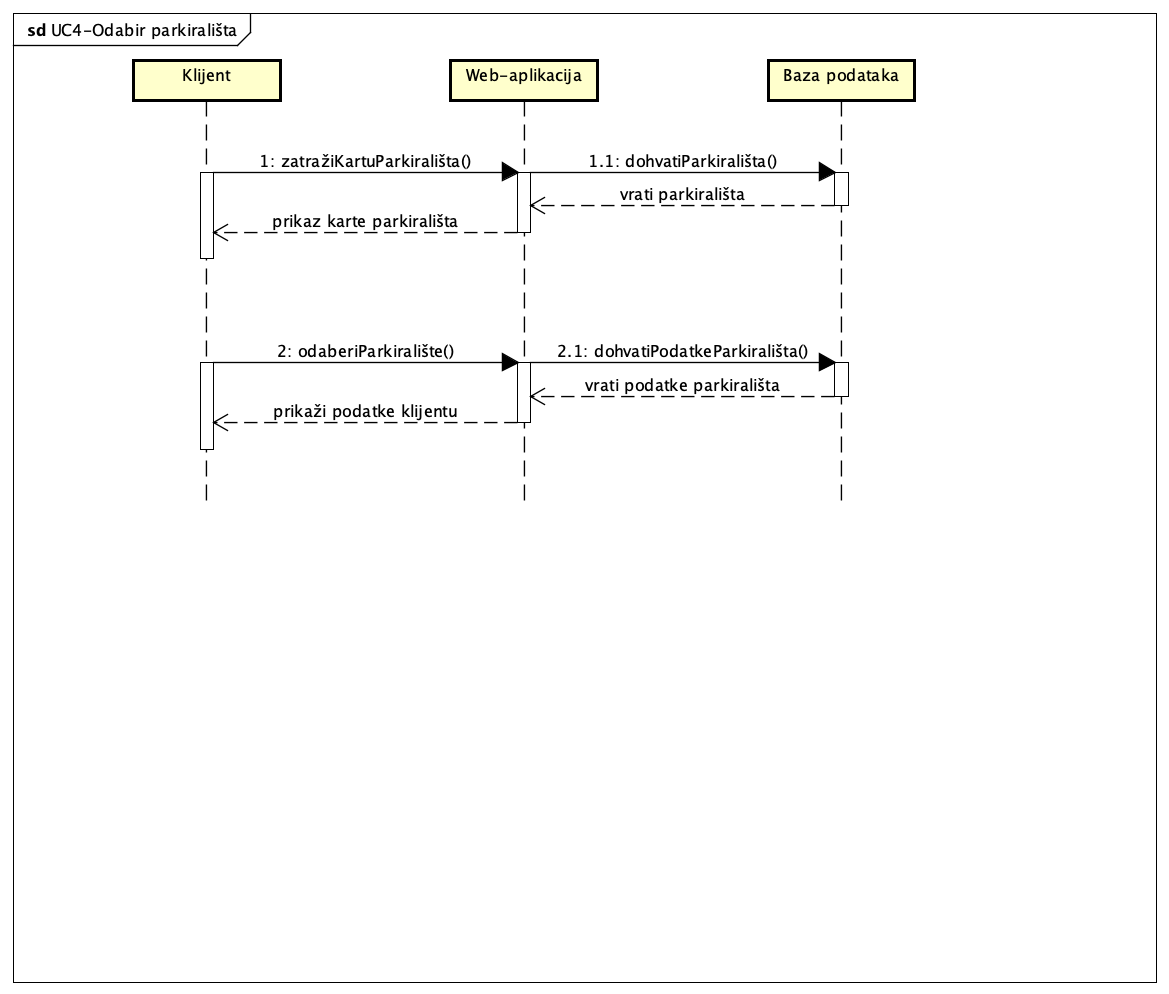
\includegraphics[width=0.7\linewidth]{../../../uc4}
				    	   \caption{Sekvencijski dijagram za UC4}
				        	\label{fig:uc4}
				       \end{figure}
				    
				    
				    
				    
				    
				    
				   \textbf{\textit{Obrazac uporabe UC5 - Rezervacija mjesta}}
				   
				   
				  
				   \textit{Klijent, nakon što je odabrao željeno parkiralište, pristupa informacijama o dostupnim parkirališnim mjestima. Aplikacija mu prikazuje kartu parkirališta s označenim slobodnim i zauzetim mjestima. Tada klijent šalje upit za odabranim mjestom, a aplikacija provjerava raspoloživost tog mjesta. Ukoliko je mjesto slobodno, klijentu se potvrđuje rezervacija, a sustav ažurira informacije o zauzetosti i evidentira rezervaciju.U slučaju da mjesta nisu slobodna, aplikacija obavještava klijenta o nedostupnosti te ga vraća na korak odabira novih mjesta ili termina.}
				   
				   \pagebreak
				   
				   
				   
				   
				    \begin{figure}[hbt!]
				    	\centering
				    	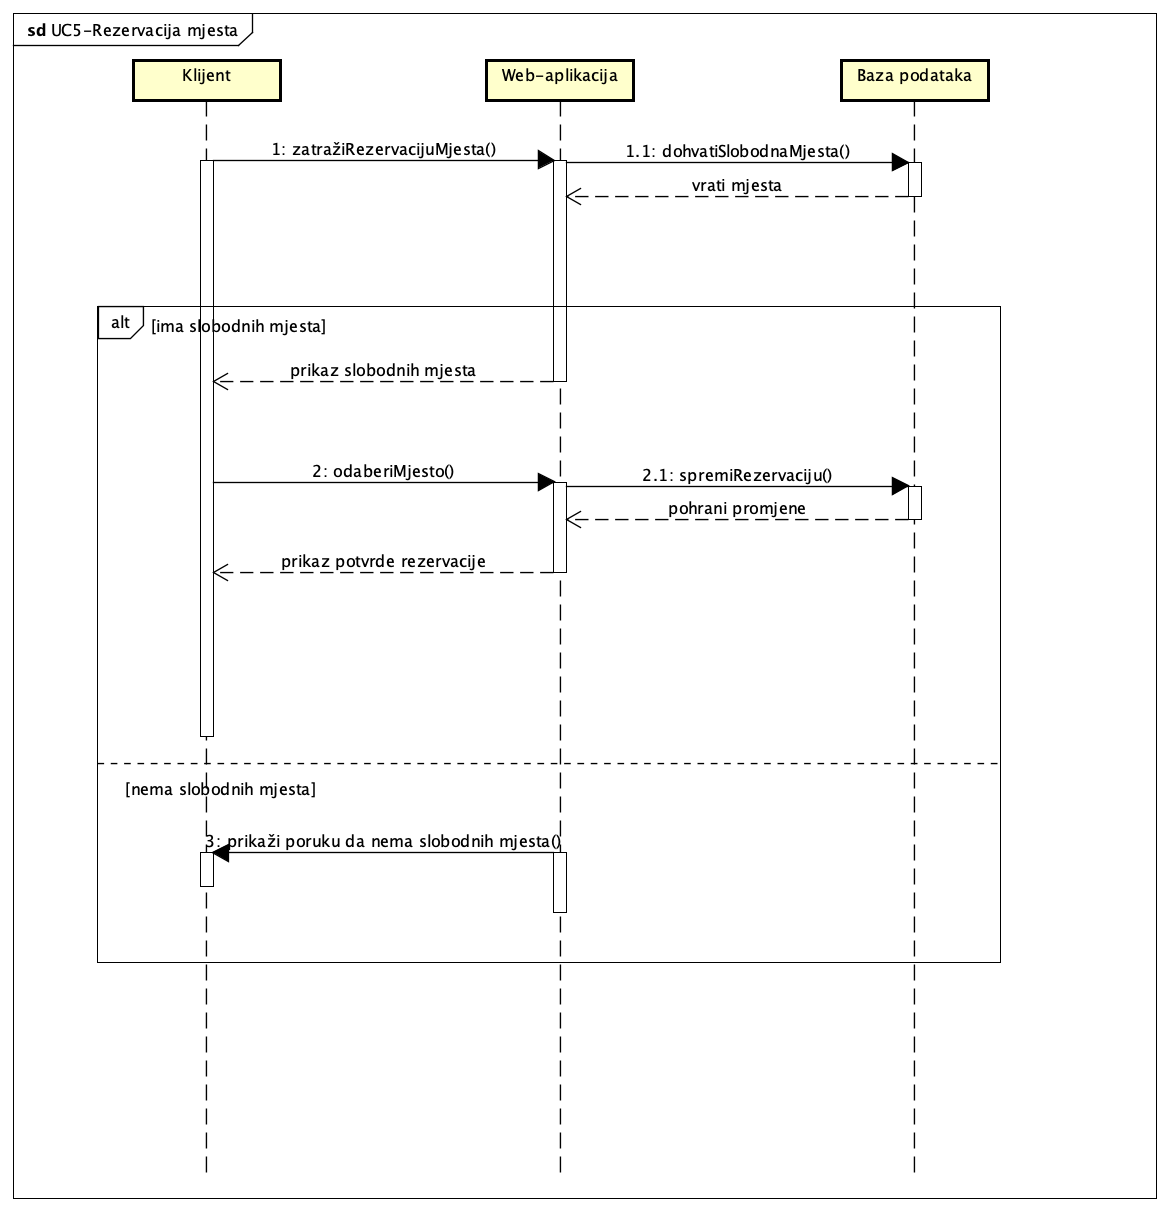
\includegraphics[width=0.7\linewidth]{../../../mjesto}
				    	\caption{Sekvencijski dijagram za UC5}
				    	\label{fig:mjesto}
				    \end{figure}
				    
				    
				    
				    
				    
				    
				    
				    
				    
				    
			     	
				    \textbf{\textit{Obrazac uporabe UC6 - Plaćanje parkirališta}}
				    				
				     \textit{Kada klijent odluči platiti parkiranje, sustav prikazuje opcije plaćanja prilikom rezervacije ili prilikom dolaska na lokaciju parkirališta. Klijent odabire željeni način plaćanja. Ako odabere plaćanje unutar aplikacije, tada aplikacija provjerava stanje novčanika. Rezervacija će se naplatiti ako klijent ima dovoljno sredstava u novčaniku, a u protivnom će mu se prikazati da treba nadoplatit svoj novčanik. Ako se odluči za opciju plaćanja parkinga na parkiralištu, tada će mu aplikacija to prihvatit i potvrdit.}
				     
				     
				     
				      \begin{figure}[hbt!]
				      	\centering
				      	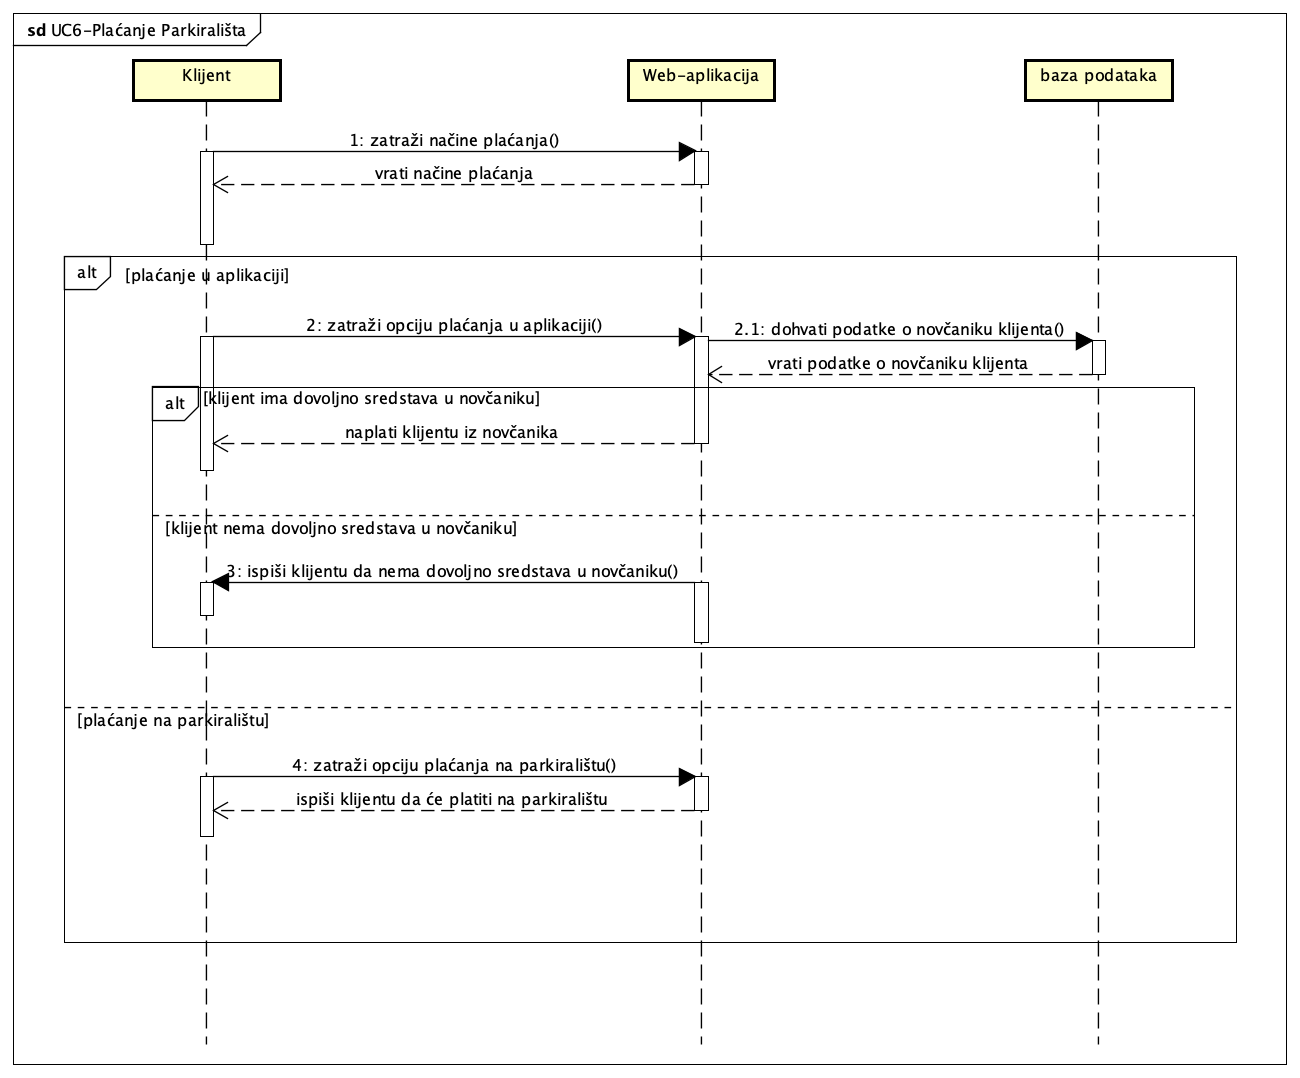
\includegraphics[width=0.7\linewidth]{../../../UC6}
				      	\caption{Sekvencijski dijagram za UC6}
				      	\label{fig:uc6}
				      \end{figure}
				      
				    
				    
				    
		   	\eject
	
		\section{Ostali zahtjevi}
		
			\textbf{\textit{dio 1. revizije}}\\
		 
			 \textit{Nefunkcionalni zahtjevi i zahtjevi domene primjene dopunjuju funkcionalne zahtjeve. Oni opisuju \textbf{kako se sustav treba ponašati} i koja \textbf{ograničenja} treba poštivati (performanse, korisničko iskustvo, pouzdanost, standardi kvalitete, sigurnost...). Primjeri takvih zahtjeva u Vašem projektu mogu biti: podržani jezici korisničkog sučelja, vrijeme odziva, najveći mogući podržani broj korisnika, podržane web/mobilne platforme, razina zaštite (protokoli komunikacije, kriptiranje...)... Svaki takav zahtjev potrebno je navesti u jednoj ili dvije rečenice.}
			 
			 
			 
	
				
						
					\chapter{Arhitektura i dizajn sustava}
			
			\begin{figure}[h]
				\centering
				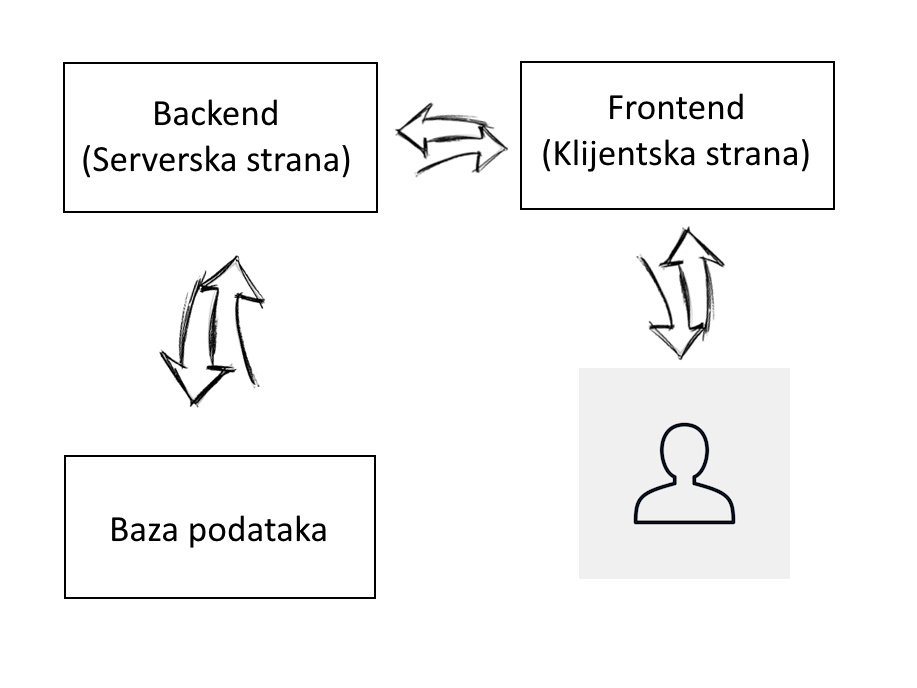
\includegraphics[width=0.8\textwidth]{slike/arhitektura-slika.jpg}
				\caption{Arhitektura sustava}
			\end{figure}
			
			{Korisnik aplikaciji pristupa putem web preglednika. Interakciju s aplikacijom ostvaruje preko korisničkog sučelja pomoću kojeg šalje zahtjeve web poslužitelju i prima odgovore.
				
				Programski jezik pomoću kojeg je ostvaren backend web aplikacije je C\#, a korišteni radni okvir je .NET. Frontend aplikacije ostvaren je programskim jezikom
				TypeScript i radnim okvirom Angular. Za razvojno okruženje backend-a odabran je Visual Studio, a frontend-a Visual Studio Code.
				
				.NET je radni okvir namijenjen stvaranju mikroservisa. Mikroservisi su arhitektura razvoja softvera koja podrazumijeva izgradnju aplikacije pomoću niza malih, nezavisnih servisa. Svaki mikroservis obavlja određeni posao i može komunicirati s drugim mikroservisima preko standardiziranih protokola. Primjena mikroservisne arhitekture u razvoju web aplikacija omogućuje agilniji pristup razvoju, povećava skalabilnost, pojednostavljuje održavanje i prilagodljivost sustava promjenama. Svaki mikroservis može se smatrati zasebnim servisom unutar web aplikacije, obavljajući specifične funkcionalnosti, poput autentifikacije, upravljanja korisnicima, poslovnih logika, itd.
				
				Arhitektura sustava temelji se na MVC (Model-View-Controller) konceptu. MVC koncept predstavlja arhitekturni obrazac koji je podržan od strane .NET radnog okvira, pružajući gotove predloške koji značajno olakšavaju razvoj web aplikacija.
				
				MVC koncept omogućuje nezavisan razvoj pojedinih dijelova aplikacije, što rezultira jednostavnijim ispitivanjem i olakšanim dodavanjem novih svojstava u sustav. Takav pristup razdvaja sustav na tri ključna dijela:
				
				\begin{itemize}
					\item \textbf{Model:} Središnja komponenta sustava koja predstavlja dinamičke strukture podataka neovisne o korisničkom sučelju. Model izravno upravlja podacima, logikom i pravilima aplikacije. Također, prima ulazne podatke od Controllera.
					
					\item \textbf{View:} Omogućuje različite prikaze istih informacija, poput grafičkog ili tabličnog prikaza podataka.
					
					\item \textbf{Controller:} Prima ulaze od korisnika i prilagođava ih za prosljeđivanje Modelu ili Viewu. Controller upravlja korisničkim zahtjevima i temeljem njih izvodi daljnju interakciju s ostalim elementima sustava. Osim posredovanja između Modela i Viewa, Controller igra ključnu ulogu u usmjeravanju tijeka aplikacije.
				\end{itemize}
				
				Ovaj trojni raspored omogućuje jasno definiranje odgovornosti svake komponente, čime se postiže modularnost sustava. Model upravlja podacima, View se brine o prezentaciji, dok Controller koordinira interakcijom između njih. Ovaj pristup često rezultira čistim, lako održivim kodom i olakšava daljnji razvoj aplikacije.
				\\
				\\
				Web aplikaciju čine tri osnovna dijela:
				\begin{itemize}
					\item \textbf{Frontend}
					\item \textbf{Backend}
					\item \textbf{Baza podataka}
				\end{itemize}
				
				Frontend se sastoji od komponenata i logike. Istu komponentu je moguće koristiti za različite namjene (engl. reusability). Angular koristi koncept komponenata i servisa koji omogućuje ponovnu upotrebu koda.  Angular koristi svojstva poput Dependency Injection i Change Detection za poboljšanje performansi. Struktura je ostvarena povezivanjem različitih komponenata unutar hijerarhijske strukture.\\
				
				Backend je ključna komponenta web aplikacije, sastavljena od sljedećih dijelova:
				
				\begin{itemize}
					\item \textbf{Programsko sučelje za reprezentacijski prijenos stanja (REST API):}
					Controller je odgovoran za obradu zahtjeva koji dolaze od korisnika ili drugih dijelova aplikacije. On prima HTTP zahtjeve, interpretira ih, te ih proslijeđuje odgovarajućim dijelovima aplikacije. Nakon obrade zahtjeva, Controller šalje odgovor korisniku, koji se sastoji od statusnog koda, tijela poruke i zaglavlja. Sadržaj u tijelu poruke predstavlja informacije koje korisnik konzumira nakon što su prikazane u web pregledniku.
					
					\item \textbf{Sloj poslovne logike (Service):}
					Service je odvojeni sloj koji sadrži poslovnu logiku aplikacije. Ovdje se obrađuju i provjeravaju podaci, izvršavaju poslovne operacije te se komunicira s ostalim dijelovima sustava. Service često služi kao posrednik između Controllera i Repository sloja. Komunikaciju sa slojem poslovne logike Controller ostvaruje pomoću umetanja ovisnosti (dependency injection). Dependency injection je obrazac prema kojemu se u određeni objekt/funkciju umeće neki drugi objekt/funkcija na koji se prvobitno spomenuti objekt/funkcija oslanja.
					
					\item \textbf{Sloj za pristup bazi podataka (Repository):}
					Repository je odgovoran za komunikaciju s bazom podataka. Ovaj sloj omogućuje izvođenje operacija poput čitanja, pisanja, brisanja i ažuriranja podataka u bazi. Koristi se SQL upitima ili ORM (Object-Relational Mapping) tehnikama za pretvaranje podataka iz relacijske baze podataka u objekte koji se koriste unutar aplikacije. Repository omogućuje komunikaciju s bazom podataka pomoću SQL-a. Objekti iz relacijske baze podataka pretvaraju se u objekte programskog jezika Java pomoću tehnike ORM.
					
				\end{itemize}
				
				Ova trostruka podjela omogućuje jasnu strukturu i odvajanje odgovornosti unutar backend-a, čineći ga modularnim i lakšim za održavanje.
				
				
			}
			
			
			
			
			
			
			
			
			\section{Baza podataka}
			
			
			
			{
				Baza podataka za aplikaciju implementirana je kao relacijska baza podataka, gdje se podaci pohranjuju u obliku redaka ili n-torki te stupaca ili atributa koji zajedno čine tablicu. Ovaj pristup omogućuje strukturiranu organizaciju podataka, gdje svaka tablica predstavlja određenu vrstu informacija, a svaki redak u tablici predstavlja konkretan zapis ili entitet. Relacijski model olakšava učinkovito upravljanje podacima, omogućuje jednostavno pretraživanje i izvođenje kompleksnih upita nad podacima, što čini bazu podataka temeljem za pouzdano čuvanje i manipulaciju informacijama u aplikaciji.}
			
			\subsection{Opis tablica}
			
			
			{
				Glavna komponenta baze je tablica User, koja se puni osobnim podacima unesenim pri registraciji korisnika u sustav. Svakom novom korisniku dodjeljuje se primarni ključ, unikatni identifikacijski broj pomoću kojeg se korisnici u bazi podataka međusobno razlikuju. Budući da korisnik može biti primatelj usluge, davatelj usluge i menadžer usluge, postoji atribut roleId koji ovisno o broju označava ulogu korisnika u sustavu. Ako je korisnik menadžer, onda je povezan na tablicu Manager preko stranog ključa userId. Tablica Manager dodatno sadrži atribut confirmedByAdmin koji opisuje je li menadžer potvrđen od strane administratora aplikacije. Kako bi korisnik opće rezervirao parkirno mjesto, postoji tablica Parking koja sadrži svoj unikatni id, id vlasnika. Svako parkiralište ima n parkirališnih mjesta koja su opisana u tablici ParkingPlace sa stranim ključem na id parkirališta u čijem su vlasništvu, te tip mjesta uz cijenu i pokazatelj zauzetosti. U sustavu baze podataka također postoji tablica Vehicle koja opisuje vozilo. Vozilo ima strani ključ na id vlasnika, te vlastiti id i naziv. Kako bi sustav rezervacija funkcionirao, postoji tablica Reservation koja povezuje korisnika, parking, parkirno mjesto, vozilo te vrijeme same rezervacije. Svaki korisnik ima svoj novčanik opisan tablicom Wallet sa stranim ključem na korisnika i količinom novca kao atributom. Na samom kraju postoji tablica Transaction koja prati uplate i isplate u sustavu. 
			}
			
			
			\begin{longtblr}[
				label=none,
				entry=none
				]{
					width = \textwidth,
					colspec={|X[6,l]|X[6, l]|X[20, l]|}, 
					rowhead = 1,
				} %definicija širine tablice, širine stupaca, poravnanje i broja redaka naslova tablice
				\hline \SetCell[c=3]{c}{\textbf{USER}}	 \\ \hline[3pt]
				\SetCell{LightGreen} user ID	& INT & jedinstveni identifikator korisnika  	\\ \hline 
				username	& VARCHAR & korisničko ime  	\\ \hline 
				password & VARCHAR & hash lozinke  \\ \hline 
				name & VARCHAR	& ime korisnika 		\\ \hline 
				surname & VARCHAR	& prezime korisnika 		\\ \hline 
				IBAN & VARCHAR(34)	& IBAN korisnika koji se koristi prilikom plaćanja 		\\ \hline 
				email & VARCHAR	& email korisnika		\\ \hline 
				is email confirmed  & BOOLEAN	& potvrda je li korisnik potvrdio svoj račun preko mail-a 		\\ \hline 
				role id & INT	& broj korisnikove uloge u sustavu \\ \hline 
				id image path & VARCHAR	& fotografija osobne iskaznice korisnika 		\\ \hline 
			\end{longtblr}
			
			\begin{longtblr}[
				label=none,
				entry=none
				]{
					width = \textwidth,
					colspec={|X[6,l]|X[6, l]|X[20, l]|}, 
					rowhead = 1,
				} %definicija širine tablice, širine stupaca, poravnanje i broja redaka naslova tablice
				\hline \SetCell[c=3]{c}{\textbf{MANAGER}}	 \\ \hline[3pt]
				\SetCell{LightBlue}user ID & INT	&  	jedinstveni identifikator korisnika koji je menadžer parkinga, strani ključ  na user ID user tablice	\\ \hline
				confirmed by admin 	& BOOLEAN & vrijednost je li korisnik potvrđen od strane administratora da je menadžer  	\\ \hline 
			\end{longtblr}
			
			\begin{longtblr}[
				label=none,
				entry=none
				]{
					width = \textwidth,
					colspec={|X[6,l]|X[6, l]|X[20, l]|}, 
					rowhead = 1,
				} %definicija širine tablice, širine stupaca, poravnanje i broja redaka naslova tablice
				\hline \SetCell[c=3]{c}{\textbf{PARKING}}	 \\ \hline[3pt]
				\SetCell{LightGreen} parking ID	& INT & jedinstveni identifikator parkinga  	\\ \hline 
				\SetCell{LightBlue} owner ID & INT & ID na korisnika vlasnika parkinga, strani ključ	\\ \hline 
				parking name & VARCHAR	& ime parkinga 		\\ \hline 
				parking description & VARCHAR	& opis parkinga, koliko ima mjesta, lokacija, je li natkriven, je li osvijetljen...		\\ \hline 
				parking photo & VARCHAR	& fotografija parkinga \\ \hline
			\end{longtblr}
			
			\begin{longtblr}[
				label=none,
				entry=none
				]{
					width = \textwidth,
					colspec={|X[6,l]|X[6, l]|X[20, l]|}, 
					rowhead = 1,
				} %definicija širine tablice, širine stupaca, poravnanje i broja redaka naslova tablice
				\hline \SetCell[c=3]{c}{\textbf{PARKING SPACE}}	 \\ \hline[3pt]
				\SetCell{LightGreen} parking space ID	& INT & jedinstveni identifikator parkirnog mjesta  	\\ \hline 
				\SetCell{LightBlue} parking ID & INT & ID na parking u čijem je vlasništvu odabrano parkirno mjesto, strani ključ	\\ \hline 
				\SetCell{LightBlue} type & INT & id vozila ciji tip odgovara odabranom parkirnom mjestu (npr: automobil, bicikl...), strani ključ	\\ \hline 
				status & ID	& status zauzetosti parkinga, vrsta podatka je integer jer je s brojem označen status parkinga	\\ \hline 
				latitude & INT	& brojčana vrijednost fizičke širine parkinga, u metrima	\\ \hline 
				longitude & INT	& brojčana vrijednost fizičke duljine parkinga, u metrima	\\ \hline 
				price & INT	& cijena parkirnog mjesta, po satu \\ \hline
			\end{longtblr}
			
			\begin{longtblr}[
				label=none,
				entry=none
				]{
					width = \textwidth,
					colspec={|X[6,l]|X[6, l]|X[20, l]|}, 
					rowhead = 1,
				} %definicija širine tablice, širine stupaca, poravnanje i broja redaka naslova tablice
				\hline \SetCell[c=3]{c}{\textbf{VEHICLE}}	 \\ \hline[3pt]
				\SetCell{LightGreen} vehicle ID	& INT & jedinstveni identifikator vozila 	\\ \hline 
				vehicle name & VARCHAR & ime vozila \\ \hline 
			\end{longtblr}
			
			\begin{longtblr}[
				label=none,
				entry=none
				]{
					width = \textwidth,
					colspec={|X[6,l]|X[6, l]|X[20, l]|}, 
					rowhead = 1,
				} %definicija širine tablice, širine stupaca, poravnanje i broja redaka naslova tablice
				\hline \SetCell[c=3]{c}{\textbf{RESERVATION}}	 \\ \hline[3pt]
				\SetCell{LightGreen} reservation ID	& INT & jedinstveni identifikator rezervacije  	\\ \hline 
				\SetCell{LightBlue} user ID & INT & ID na korisnika koji je napravio rezervaciju, strani ključ	\\ \hline 
				reservation date & DATETIME & datum i vrijeme rezervacije	\\ \hline 
				duration & TIME	& vremenska duljina rezervacije, u satima	\\ \hline 
				\SetCell{LightBlue}vehicle type & INT	& tip vozila na čije ime glasi rezervacija, strani ključ na tablicu vehicle	\\ \hline 
				\SetCell{LightBlue} parking space id & INT	& jedinstveni identifikator koje je točno parkirno mjesto rezervirano, strani ključ	\\ \hline 
				repeating & BOOLEAN	& vrijednost koja pokazuje treba li se rezervacija periodički ponavljati (na dnevnoj, tjednoj ili mjesečnoj razini...) \\ \hline
			\end{longtblr}
			
			\begin{longtblr}[
				label=none,
				entry=none
				]{
					width = \textwidth,
					colspec={|X[6,l]|X[6, l]|X[20, l]|}, 
					rowhead = 1,
				} %definicija širine tablice, širine stupaca, poravnanje i broja redaka naslova tablice
				\hline \SetCell[c=3]{c}{\textbf{TRANSACTION}}	 \\ \hline[3pt]
				\SetCell{LightGreen} transaction ID	& INT & jedinstveni identifikator transakcije 	\\ \hline 
				\SetCell{LightBlue} user ID	& INT & ID na korisnika koji je obavio transakciju, strani ključ 	\\ \hline 
				type & INT & tip transakcije \\ \hline 
				amount & FLOAT & količina novca koji je prošao kroz transakciju \\ \hline 
			\end{longtblr}
			
			\begin{longtblr}[
				label=none,
				entry=none
				]{
					width = \textwidth,
					colspec={|X[6,l]|X[6, l]|X[20, l]|}, 
					rowhead = 1,
				} %definicija širine tablice, širine stupaca, poravnanje i broja redaka naslova tablice
				\hline \SetCell[c=3]{c}{\textbf{WALLET}}	 \\ \hline[3pt]
				\SetCell{LightGreen} wallet ID	& INT & jedinstveni identifikator novčanika 	\\ \hline 
				\SetCell{LightBlue} user ID	& INT & ID na korisnika u čijem je vlasniku virtualni novčanik, strani ključ 	\\ \hline 
				balance & FLOAT & količina novca koji se nalazi u novčaniku \\ \hline 
			\end{longtblr}
			
			
			
			\subsection{Dijagram baze podataka}
			
			\begin{figure}[h]
				\centering
				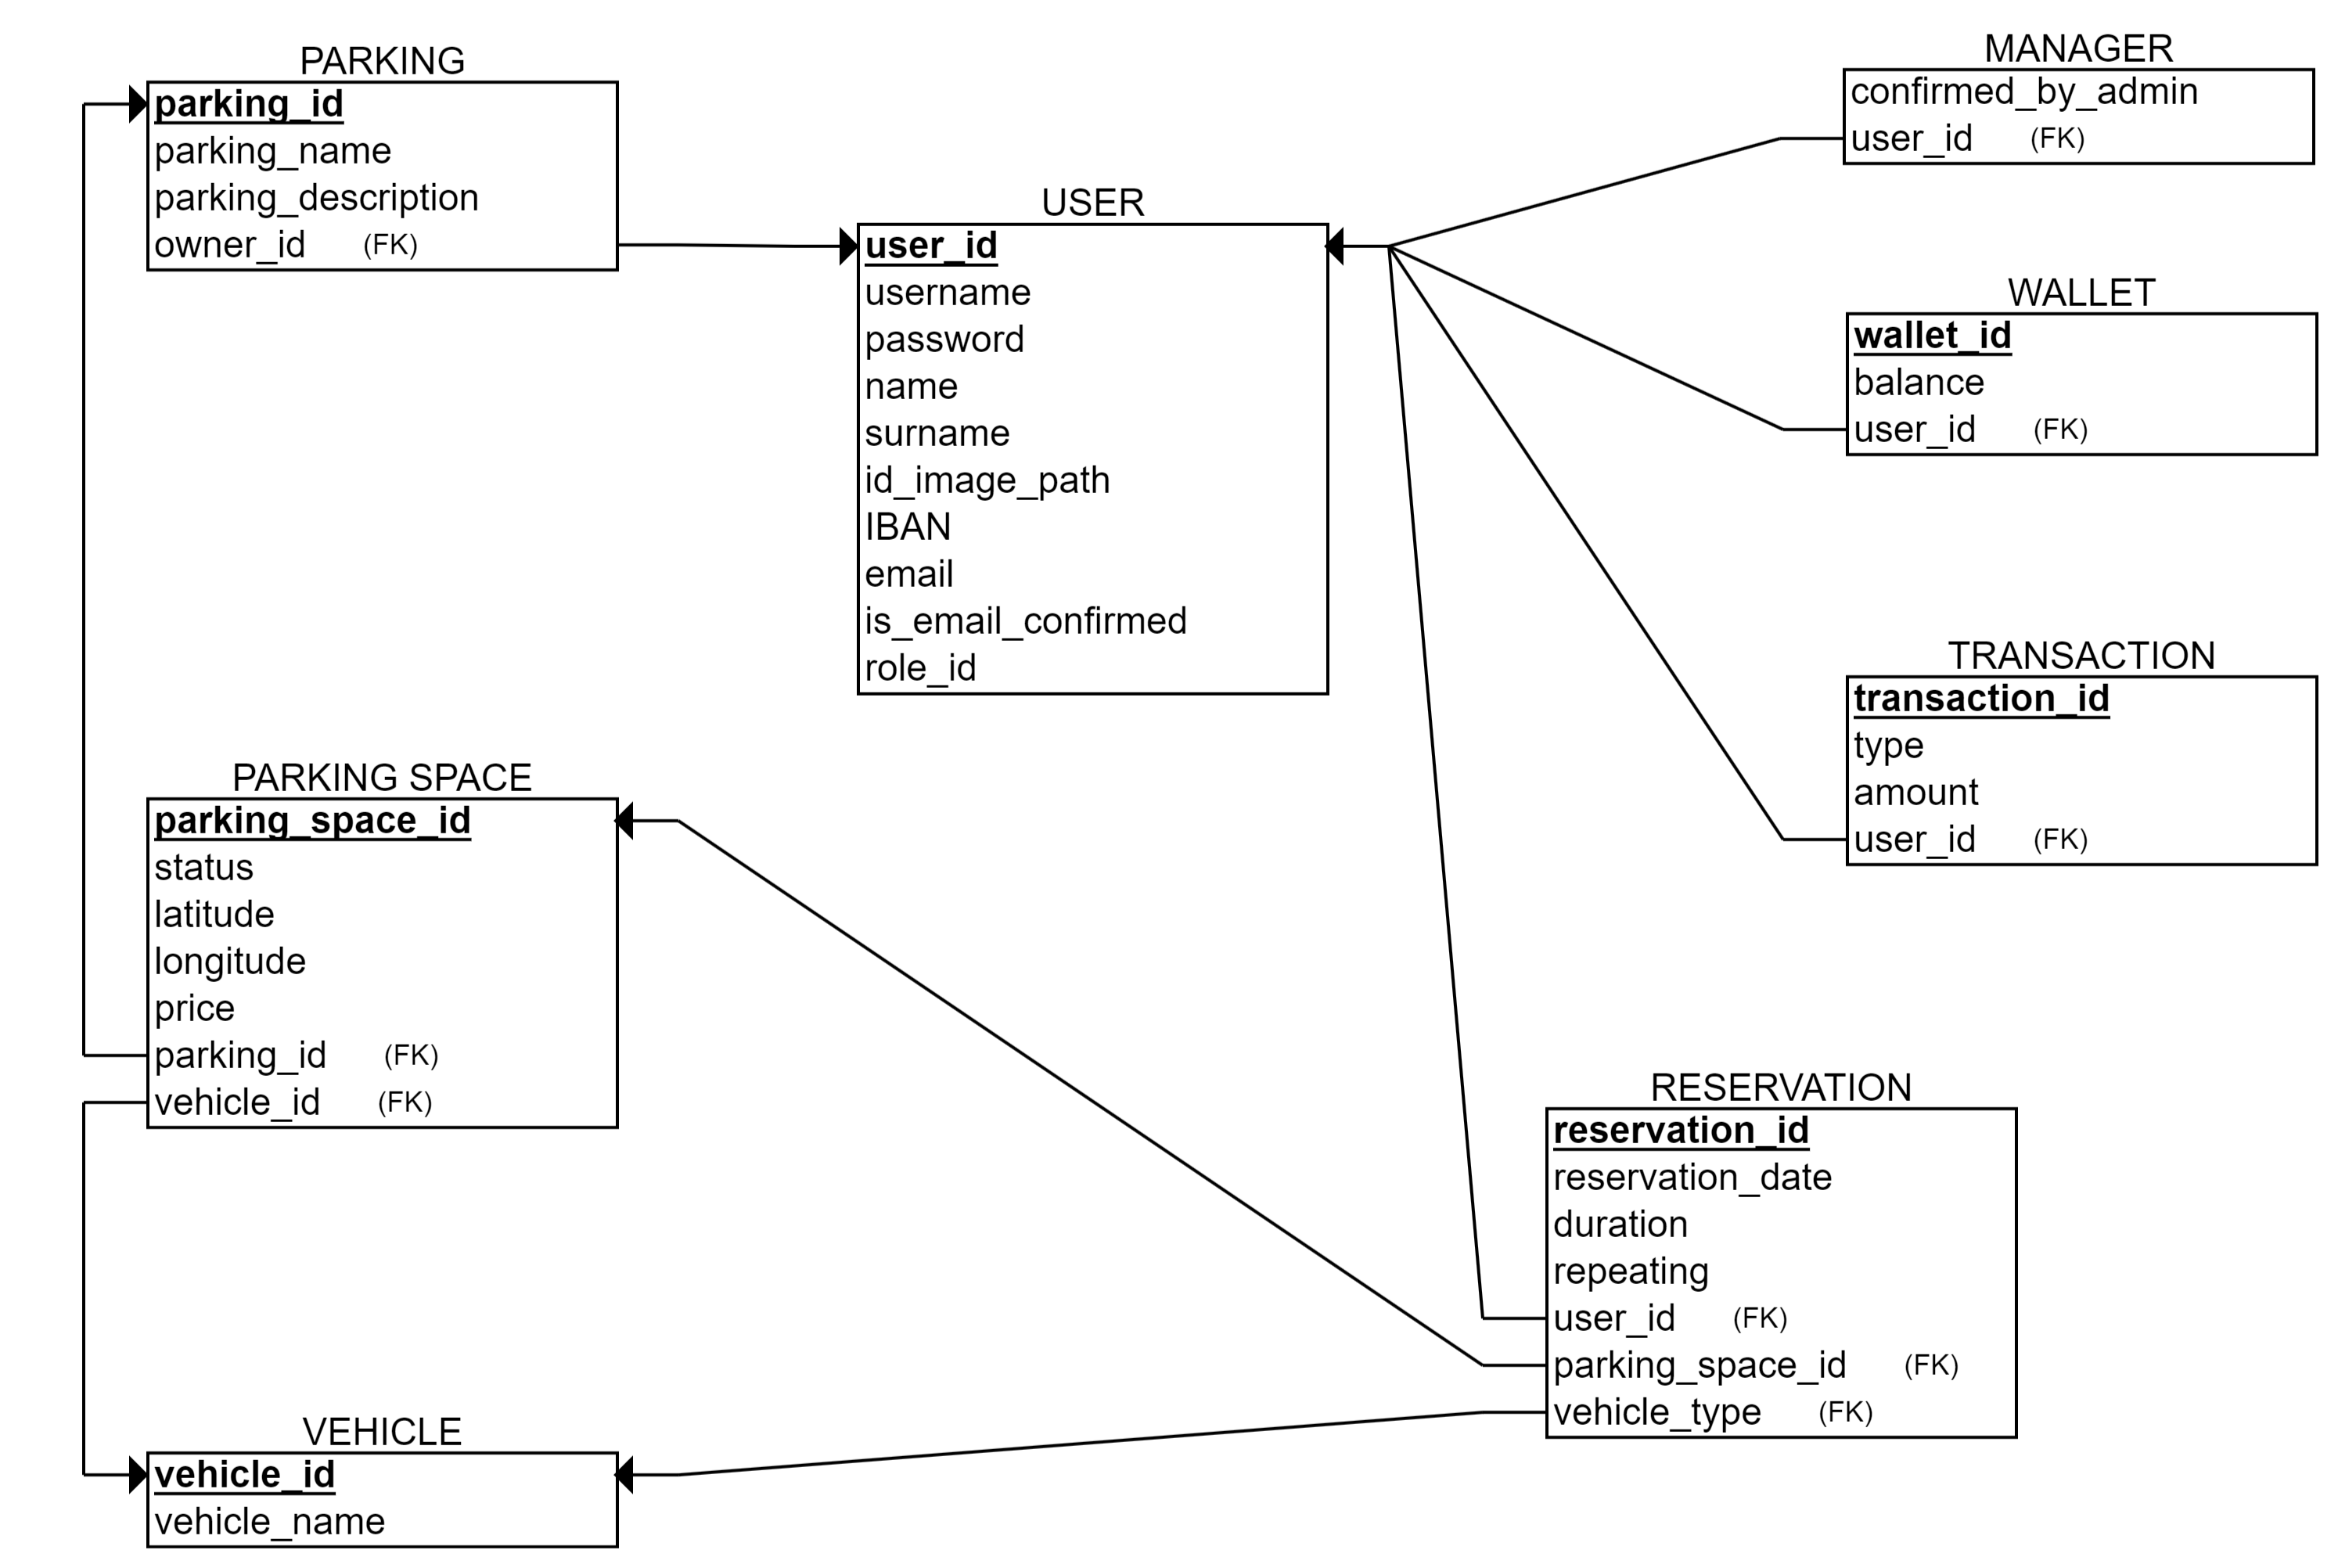
\includegraphics[width=0.8\textwidth]{slike/baza-slika.png}
				\caption{ER dijagram baze podataka}
			\end{figure}
			
			
			
			
		\section{Dijagram razreda} 
			
			{ Na slikama su prikazani razredi („Class“) koji su korišteni za implementaciju backend-a. Na slici \ref{fig:controllers} su prikazani razredi koji nasljeđuju Controller razred. Sve funkcije implementirane u Controller razredu vraćaju IActionResult (podatke i odgovarajući kod). Također, sve funkcije ne komuniciraju direktno s bazom podataka nego pozivaju funkcije iz određenih servisa koji imaju implementiranu tu funkcionalnost. Funkcije u kontrolerima kao parametre primaju odgovarajući model. }
			
			\begin{figure}[h]
				\centering
				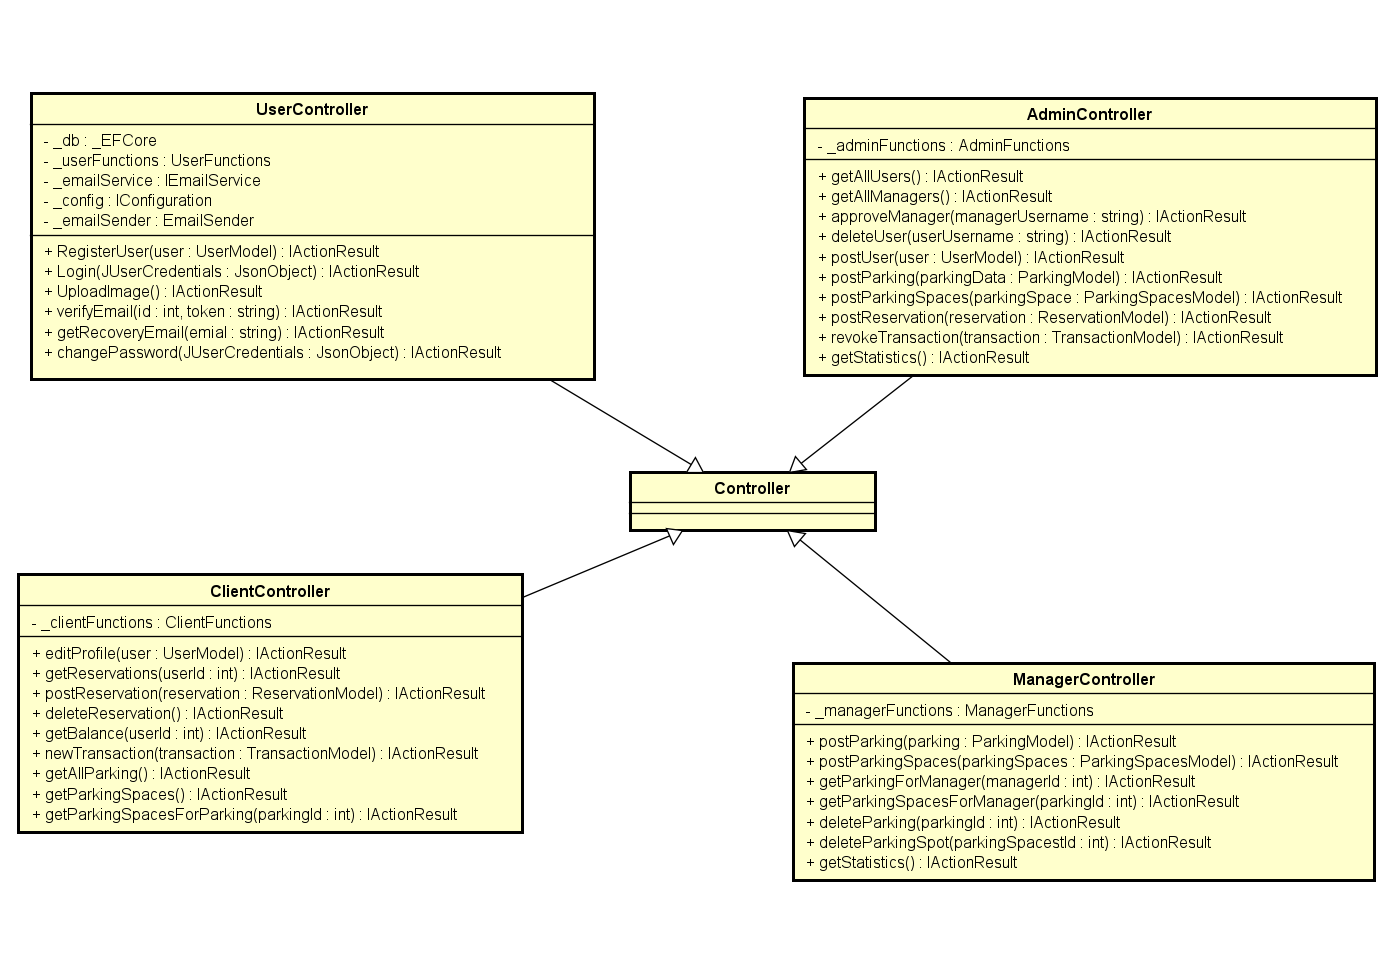
\includegraphics[width=\textwidth,keepaspectratio]{slike/progi4_1.png}
				\caption{dio Controllers}
				\label{fig:controllers}
			\end{figure}
			\pagebreak
			
			{Modeli razreda odražavaju strukturu baze podataka unutar aplikacije. Metode implementirane unutar tih razreda izravno komuniciraju s bazom podataka kako bi dobile tražene informacije. Razred User predstavlja generičnog korisnika aplikacije koji se može registrirati. Na taj razred referira se razred Manager (jer je svaki Manager ujedno i User).}
			
				\pagebreak
			
			\begin{figure}[h]
				\centering
				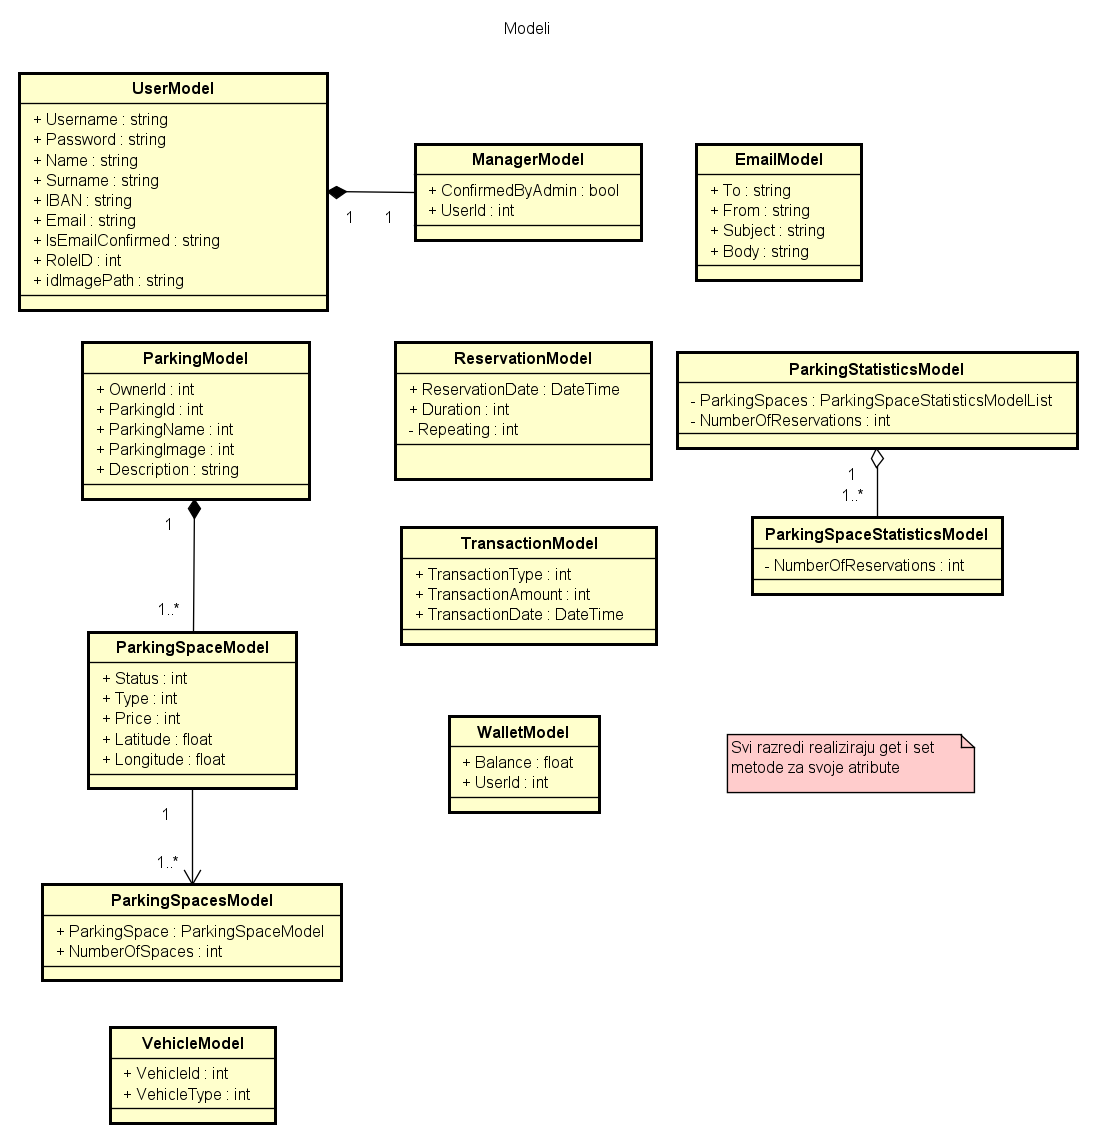
\includegraphics[width=\textwidth,keepaspectratio]{slike/progi_1.png}
				\caption{dio Models}
				\label{fig:models}
			\end{figure}
			
				\pagebreak
		
			
			\begin{figure}[h]
				\centering
				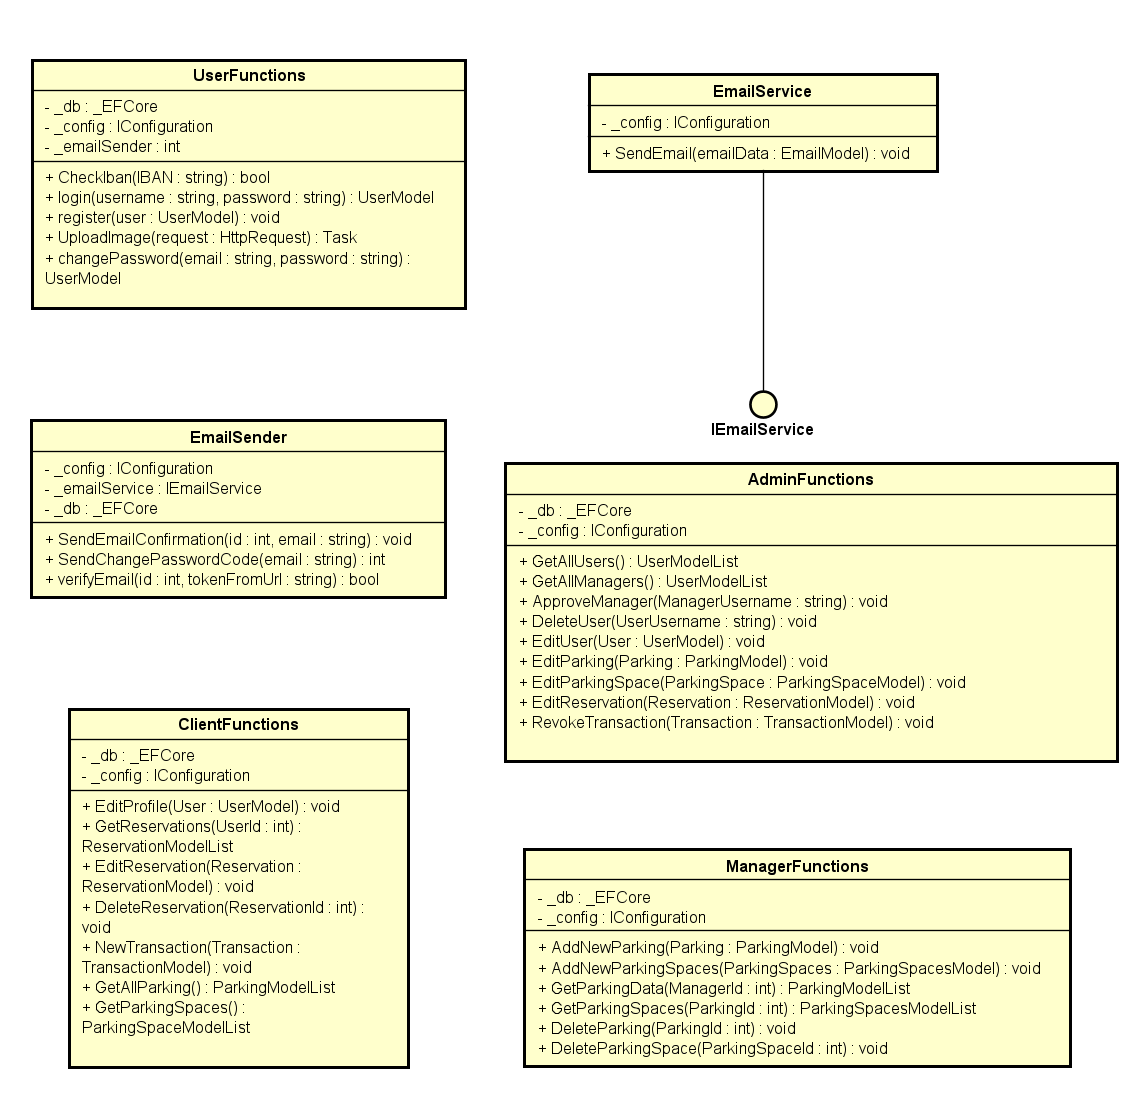
\includegraphics[width=\textwidth,keepaspectratio]{slike/progi3_1.png}
				\caption{dio Services}
				\label{fig:services}
			\end{figure}
			
				\pagebreak
			
			{U dijagramu razreda na slici \ref{fig:services} prikazani je dio servisa. Svi servisi kao svoj atribut, između ostalih, imaju instancu objekta \_EFCore koji predstavlja kontekst za bazu podataka i instancu IConfiguration objekta koji služi za dohvaćanje konstanti. Funkcije definirane u pojedinom razredu dohvaćaju, mijenjaju i dodaju podatke u bazu podataka i manipuliraju podacima koje vraćaju kontroleru koji šalje nazad do korisnika.}
				\pagebreak
			
			\begin{figure}[h]
				\centering
				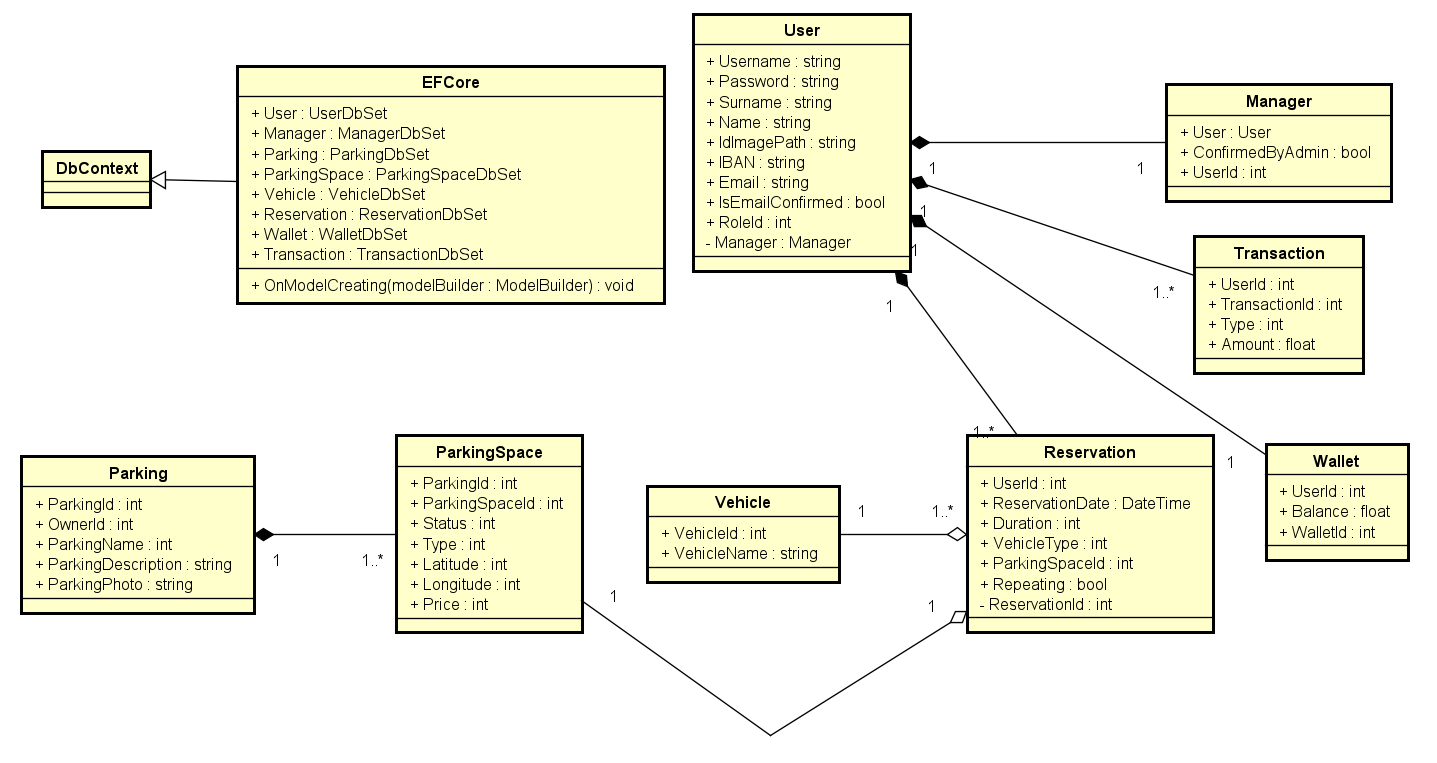
\includegraphics[width=\textwidth,keepaspectratio]{slike/progi2_1.png}
				\caption{Reprezentacija baze podataka}
				\label{fig:repr}
			\end{figure}
			
		
			
			\pagebreak
		
		\section{Dijagram stanja}
			
			
			
			{Dijagram stanja prikazuje stanja objekta te prijelaze iz jednog stanja u drugo temeljene na događajima. Na slici je prikazan dijagram stanja za registriranog korisnika bilo kao admin ili korisnik. Nakon prijave admina kao korisničkog admina prikazuje mu se početna stranica na kojoj može pregledati sve registrirane korisnike te izmjenjivati njihove podatke. Ako se admin prijavi kao vlasnik parkinga prikazuje mu se početna stranica na kojoj može unositi podatke o parkirnom mjestu, podatke o dostupnosti parkirnog mjesta te dohvatiti statistiku grafa o parkingu. Korisnik s druge strane kada se prijavi na svojoj početnoj stranici pregledava parkirališta, odabire parkirno mjesto te odabire plaćanje dolaskom na parking ili plaćanje karticom te sredstvima iz novčanika. }
			
		
			\begin{figure}[h]
				\centering
				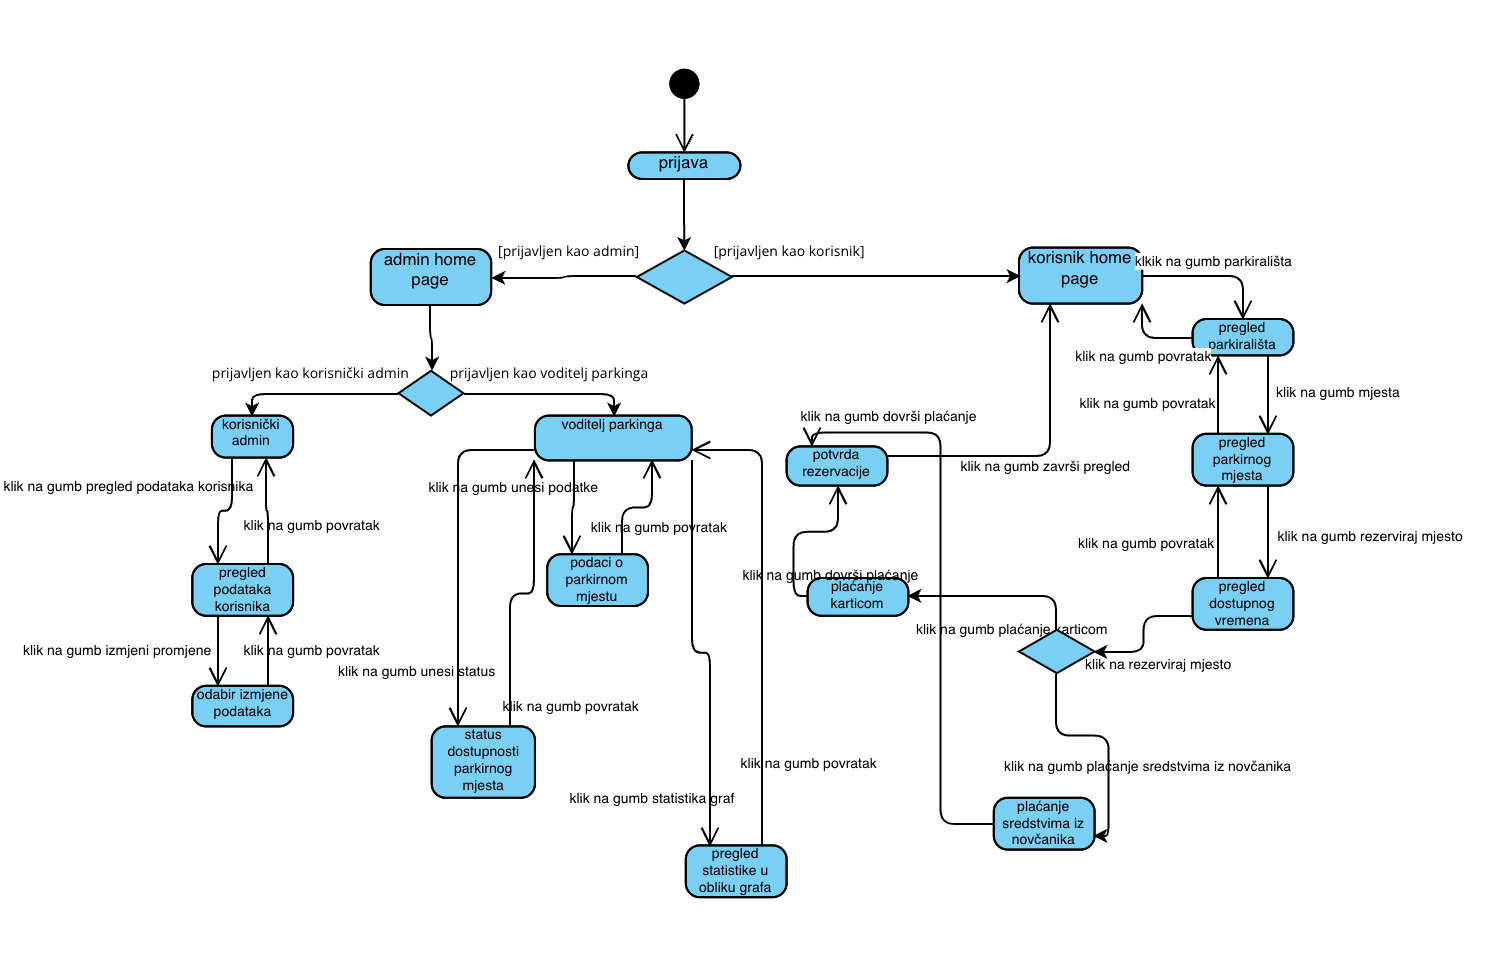
\includegraphics[width=\textwidth,keepaspectratio]{slike/DijagramStanjacopyy.png}
				\caption{Dijagram stanja}
				\label{fig:DijagramStanjacopyy}
			\end{figure}
			
			
			
			\eject 
		
		\section{Dijagram aktivnosti}
			
			
			
			 {Dijagram aktivnosti koristi se za opis modela upravljačkog ili podatkovnog toka. Nije namijenjen modeliranju događaja potaknutog ponašanja. U modeliranju upravljačkog toka, svaki sljedeći korak slijedi nakon završetka prethodnog, pri čemu se naglašava jednostavnost. Na slici je prikazan dijagram aktivnosti koji opisuje proces rezerviranja parkirnog mjesta. Korisnik nakon uspješne prijave odabire parking, parkirališno mjesto, datum i vrijeme. Zatim mu se prikazuju opcije plaćanja te rezervacije gdje nakon uspješne transakcije korisniku se potvrđuje rezervacija.}
			
			\begin{figure}[hbt!]
				\centering
				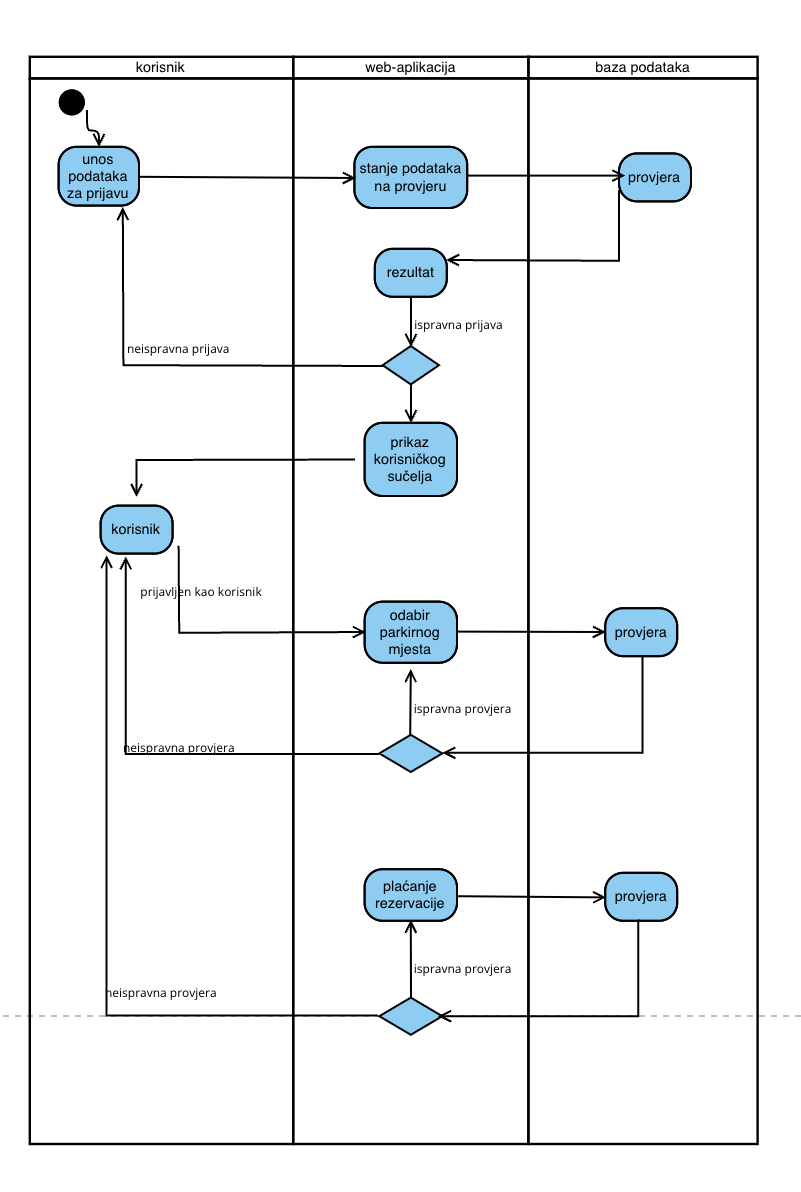
\includegraphics[width=0.7\linewidth]{slike/DijagrammmAktivnosti.png}
				\caption{Dijagram aktivnosti}
				\label{fig:DijagrammmAktivnosti}
			\end{figure}
			
			
			\eject
		\section{Dijagram komponenti}
		
			
		
			 {Dijagram komponenti, prikazan na slici, ilustrira organizaciju i međusobnu povezanost komponenti, unutarnju strukturu te odnose s okolinom. Sustav je dostupan putem dva različita sučelja. Sučeljem za dohvat HTML, CSS i JS datoteka pristupaju datoteke koje pripadaju frontend dijelu aplikacije. Router je komponenta koja, na temelju upita s URL-a, određuje koja datoteka će biti poslužena na sučelju. Frontend se sastoji od niza JavaScript datoteka grupiranih u logičke cjeline nazvane prema tipovima korisnika koji im pristupaju. Sve JavaScript datoteke ovise o Angular biblioteci, iz koje se pozivaju gotove komponente poput gumba, obrazaca i slično.}
			 
			 {Sučeljem za dohvat JSON podataka pristupa se REST API komponenti, koja poslužuje podatke pripadajuće backend dijelu aplikacije. EntityFrameworkCore je odgovoran za dohvaćanje tablica iz baze podataka putem SQL upita. Podaci koji stižu iz baze šalju se dalje MVC arhitekturi u obliku DTO (Data Transfer Object).}
			 
			
			 
			 \begin{figure}[h]
			 	\centering
			 	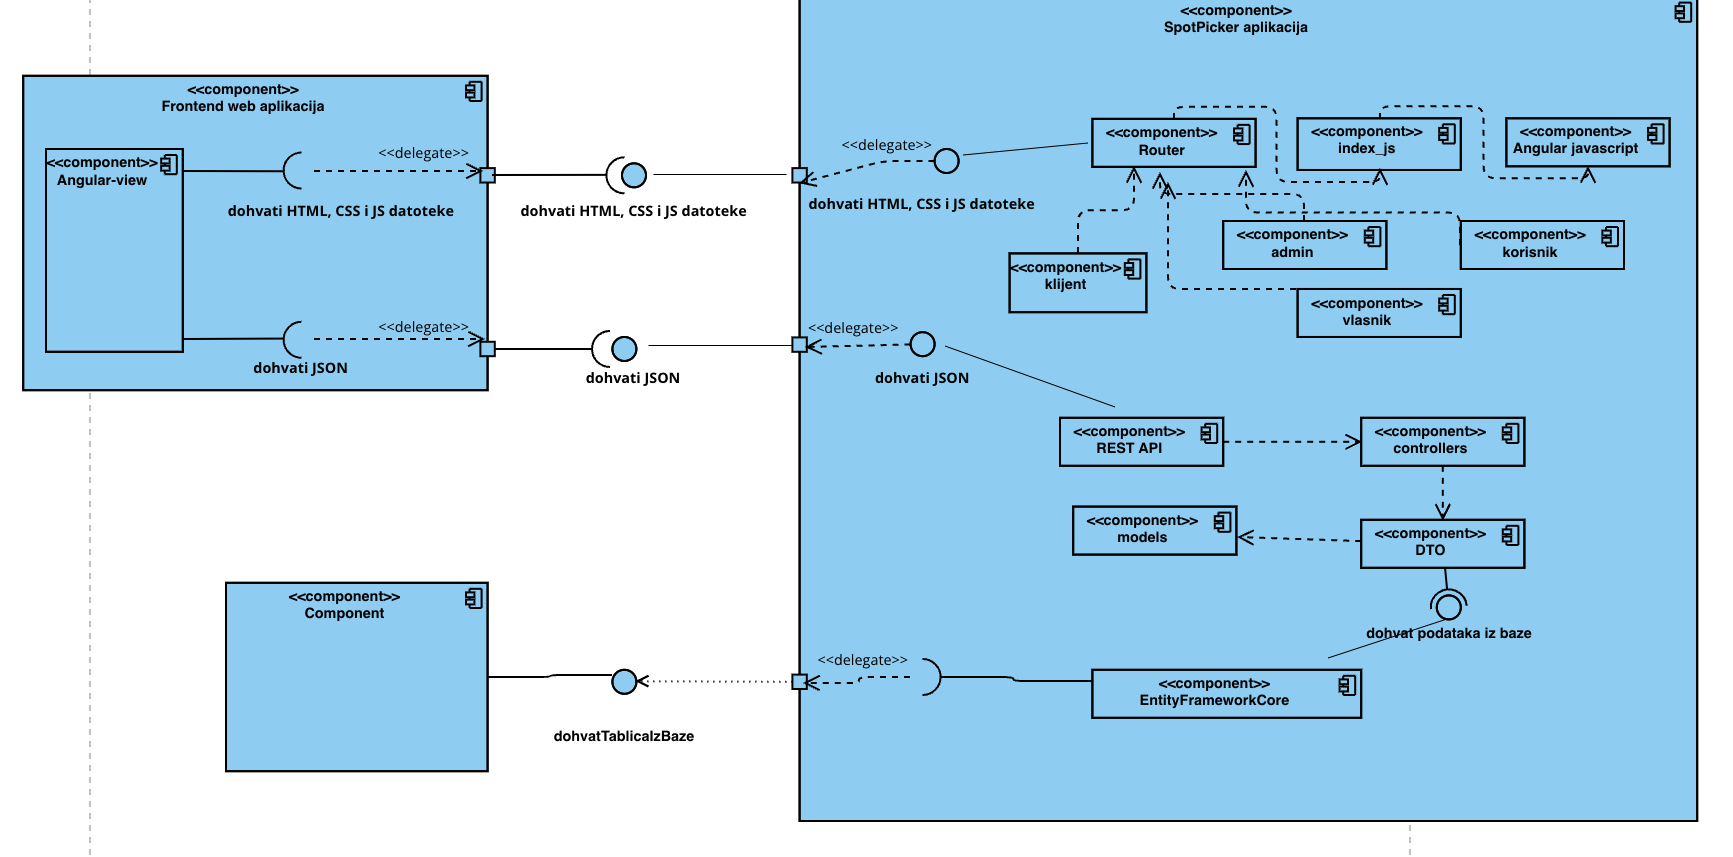
\includegraphics[width=\textwidth,keepaspectratio]{slike/DijagramKomponenti.png}
			 	\caption{Dijagram komponenti}
			 	\label{fig:DijagramKomponenti}
			 \end{figure}
			 
	\chapter{Implementacija i korisničko sučelje}
		
		
		\section{Korištene tehnologije i alati}
		
		
			
			 {Za međusobnu komunikaciju unutar tima korišten je Discord u kojem su članovi tima bili podijeljeni u nekoliko kanala kako bi se organizirali različiti dijelovi projekta. Također za svojevrsnu komunikaciju upotrebljavan je i GitHub što je jedna od najpoznatijih platformi koja omogućuje programerima da imaju repozitorije u kojima zatim mogu stvarati, pohranjivati i upravljati svojim kodovima i projektima. Također moguće je pratiti svaku promjenu. Prilikom izrade projekta GitHub je služio kako bi bila olakšana međusobna komunikacija te kako bi na jednom mjestu bilo dostupno sve što se radi na projektu u svakom trenutku.}
			 
			 {Za izradu dokumentacije korišten je sustav za uređivanje teksta LaTex. Ovaj markup jezik se najčešće koristi za izradu znanstvene i tehničke publikacije. Njegove prednosti su lakoća formatiranja velikih datoteka što olakšava i skraćuje vrijeme koje bi se potrošilo na uređivanje samog dokumenta. Prilikom izrade UML dijagrama korišten je Astah UML alat za modeliranje UML dijagrama. Poznat je po tome što je vrlo jednostavan za učenje i korištenje. Također brži je od Excela i drugih alata za crtanje. Astah je primijenjen prilikom izrade dijagrama obrazaca uporabe, sekvencijskih dijagrama, dijagrama baze podataka,  dijagrama razreda, stanja, aktivnosti, komponenti te dijagram razmještaja.Za izradu frontenda korišten je Angular te jezik Typescript dok su za backend korišteni .NET Framework i jezik C}
			 
			 
			 
			 {Angular je platforma tj. okvir (eng. Framework) koji služi za razvijanje web aplikacija pomoću TypeScript-a i HTML-a. Kako bi se mogao koristiti Angular potrebno je prethodno instalirati NPM te Node.js. Prednost Angular-a je kod koji je lako čitljiv te koji se može ponovno iskoristiti, također dobra je tehnologija za rad u timu s obzirom da omogućuje usporedan samostalan rad. Radni okvir .NET Framework namijenjen je za izgradnju i izvođenje aplikacija. Korišteni su i Visual Studio Code i Visual Studio. To su integrirana razvojna okruženja (eng. IDE). Koriste se kao platforma za uređivanje izvornog koda te platforma za  pokretanje koja se može koristiti za uređivanje, debugiranje, izgradnju koda i samo objavljivanje aplikacije.}
			 
			 
			 {PGAdmin je korisničko grafičko sučelje iskorišteno za interakciju sa Postgres-om prilikom izrade baze podataka dok je EntityFramework korišten kao poveznica baze podataka i backend-a. Za dohvat početne informacije o parkirališnim mjestima upotrebljeno je aplikacijsko programsko sučelje Overpass, a za mapu je iskorišten Open Street Map. Također korišten je Nominatim koji služi za pretvaranje koordinata u adresu te OSRM Demo API koji koristi algoritme usmjeravanja za izračun i pronalazak najkraćeg puta do odredišta.}
			
			\begin{enumerate}
				
				
				\item   \url{https://discord.com/}
				
				\item   \url{https://github.com/}
				
				\item   \url{https://www.latex-project.org/}
				
				\item  \url{https://astah.net/products/astah-uml/}
				
				\item   \url{https://angular.io/}
				
				\item   \url{https://dotnet.microsoft.com/en-us/learn/dotnet/what-is-dotnet-framework}
				
				\item   \url{https://visualstudio.microsoft.com/}
				
				\item   \url{https://www.pgadmin.org/}
				
				\item   \url{https://learn.microsoft.com/en-us/aspnet/entity-framework}
				
				\item   \url{https://hrbrmstr.github.io/overpass/}
				
				\item   \url{https://www.openstreetmap.org/#map=7/44.523/16.460}
				
				\item   \url{https://nominatim.openstreetmap.org/ui/search.html}
				
				\item   \url{https://project-osrm.org/docs/v5.5.1/api/#introduction}
				
				
			\end{enumerate}
			
			\eject 
		
	
		\section{Ispitivanje programskog rješenja}
			
			
			
			 {Opisujemo provedbu ispitivanja implementiranih funkcionalnosti na razini komponenti i na razini cijelog sustava s prikazom odabranih ispitnih slučajeva.}
	
			
			\subsection{Ispitivanje komponenti}
			
			\textbf{DistanceFunctionTest}
			
			{Pri stvaranju instantne rezervacije traži se parkirno mjesto koje je najbliže traženoj destinaciji. Pri tome odlučili smo koristiti Haversinovu formulu. Za ovaj test odabrali smo pouzdan primjer za koji znamo točan odgovor te testirali vraća li funkcija ispravnu vrijednost:}
			
			\begin{figure}[h]
				\centering
				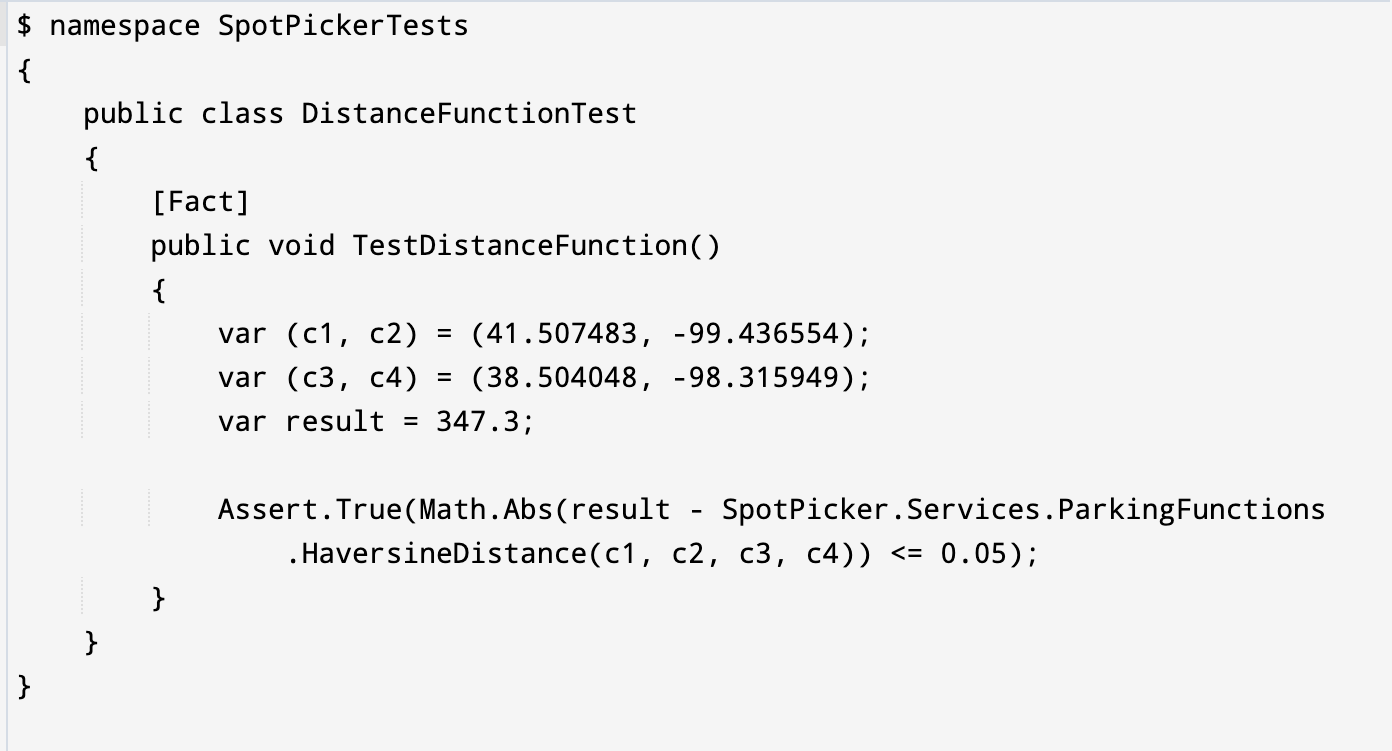
\includegraphics[width=\textwidth,keepaspectratio]{slike/kod1.png}
				\caption{DistanceFunctionTest}
				\label{fig:kod1}
			\end{figure}
			
			
			\textbf{IBanFunctionTest}
			
			{Pri mijenjanju IBAN-a od strane admina ili registraciji provjerava se validnost unesenog IBAN-a. Zato testiramo funkciju koja to provjerava pomoću ispravnog i neispravnog IBAN-a:}
			
			
		
			\begin{figure}[hbt!]
				\centering
				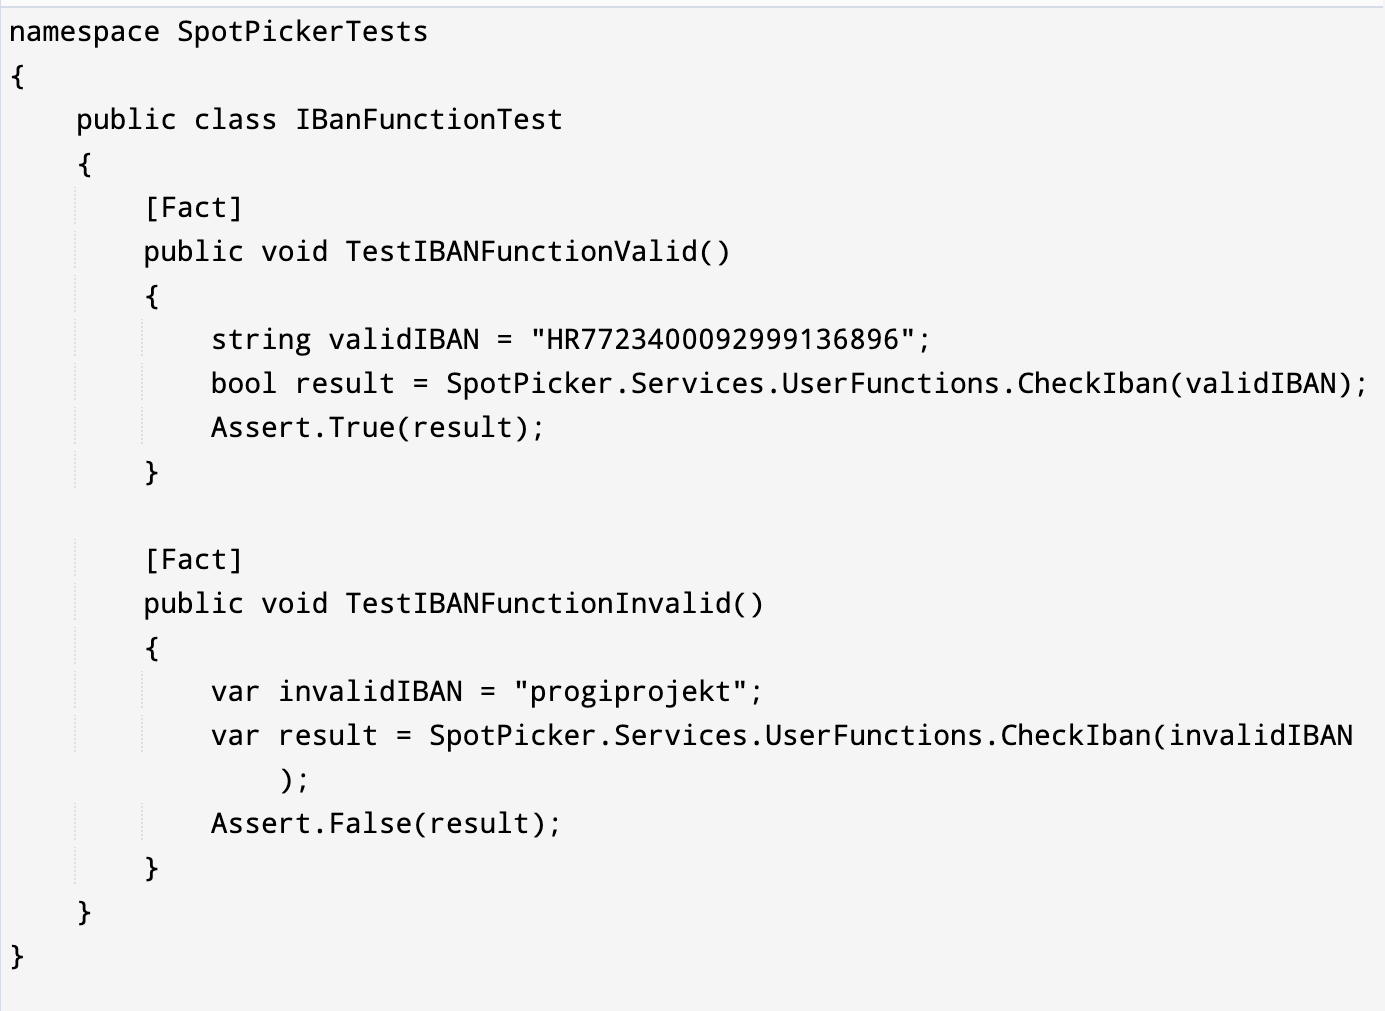
\includegraphics[width=0.7\linewidth]{slike/kod2.png}
				\caption{IBanFunctionTest}
				\label{fig:kod2}
			\end{figure}
			
			
			\textbf{PasswordRegexTest}
			
			{Pri registraciji unosi se lozinka, minimalna duljina je 8 znakova, uključujući minimalno jednu znamenku, zato testiramo tu funkciju s nekoliko primjera:}
			
			
			
			
			\begin{figure}[hbt!]
				\centering
				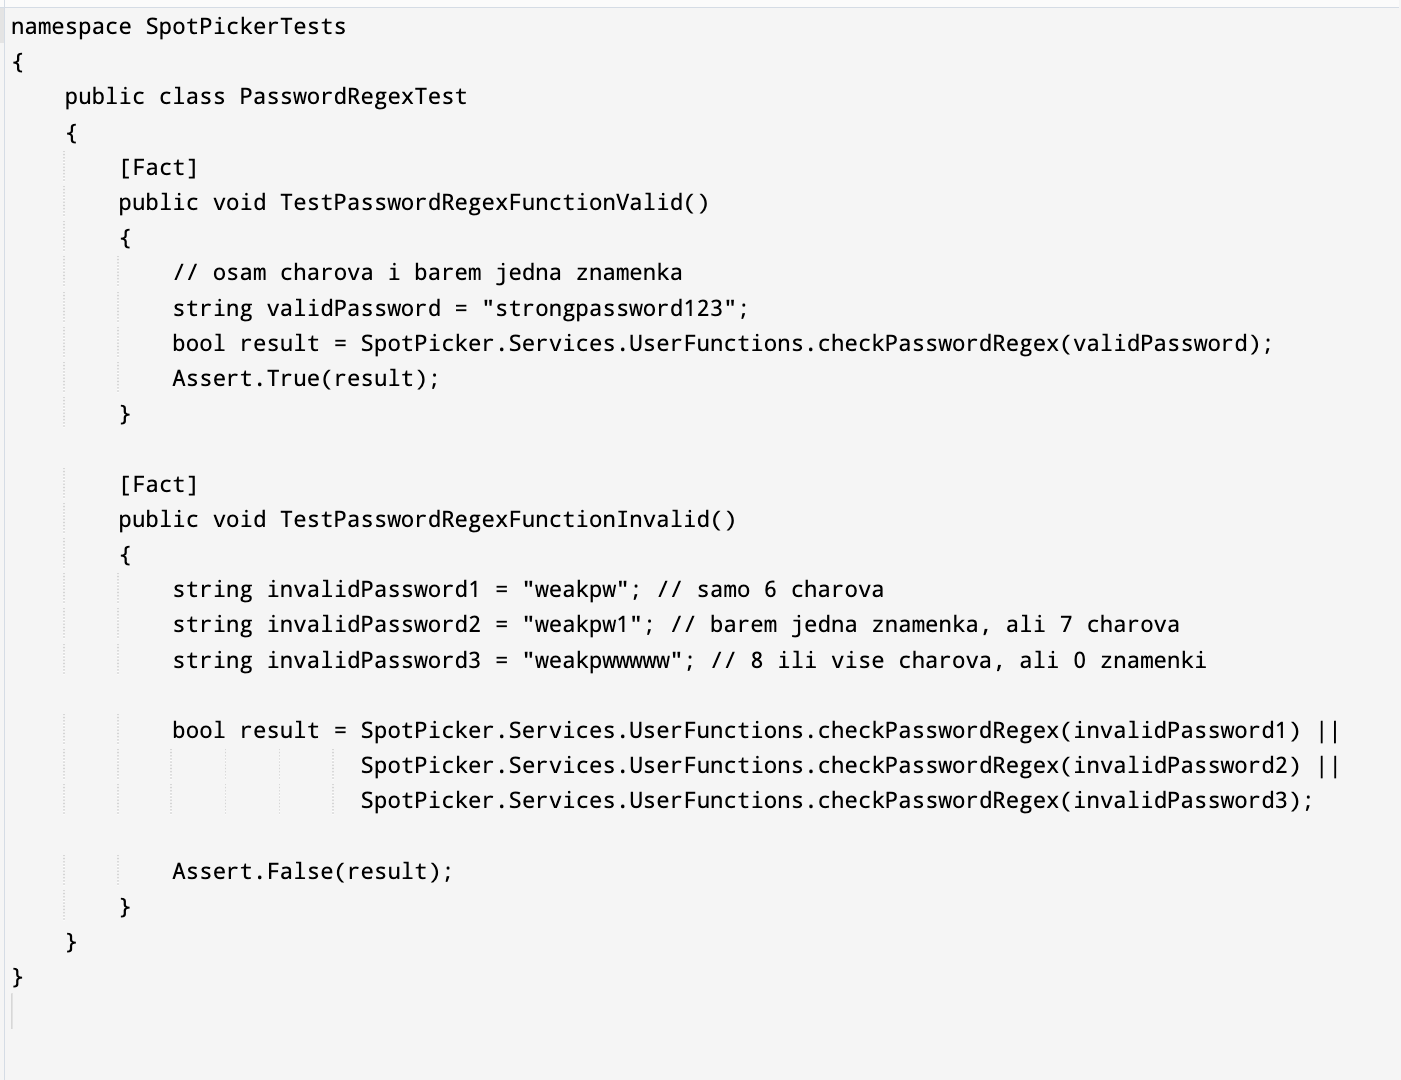
\includegraphics[width=0.7\linewidth]{slike/kod3.png}
				\caption{PasswordRegexTest}
				\label{fig:kod3}
			\end{figure}
			
			
			
		
			
			
			
			
			\subsection{Ispitivanje sustava}
			
			 \textbf{LoginTest}
			 
			 {Ovo je sistem test koji testira funkcionira li login (ulogira se u adminov profil):}
			 
			
			 
			
			 
			 \begin{figure}[hbt!]
			 	\centering
			 	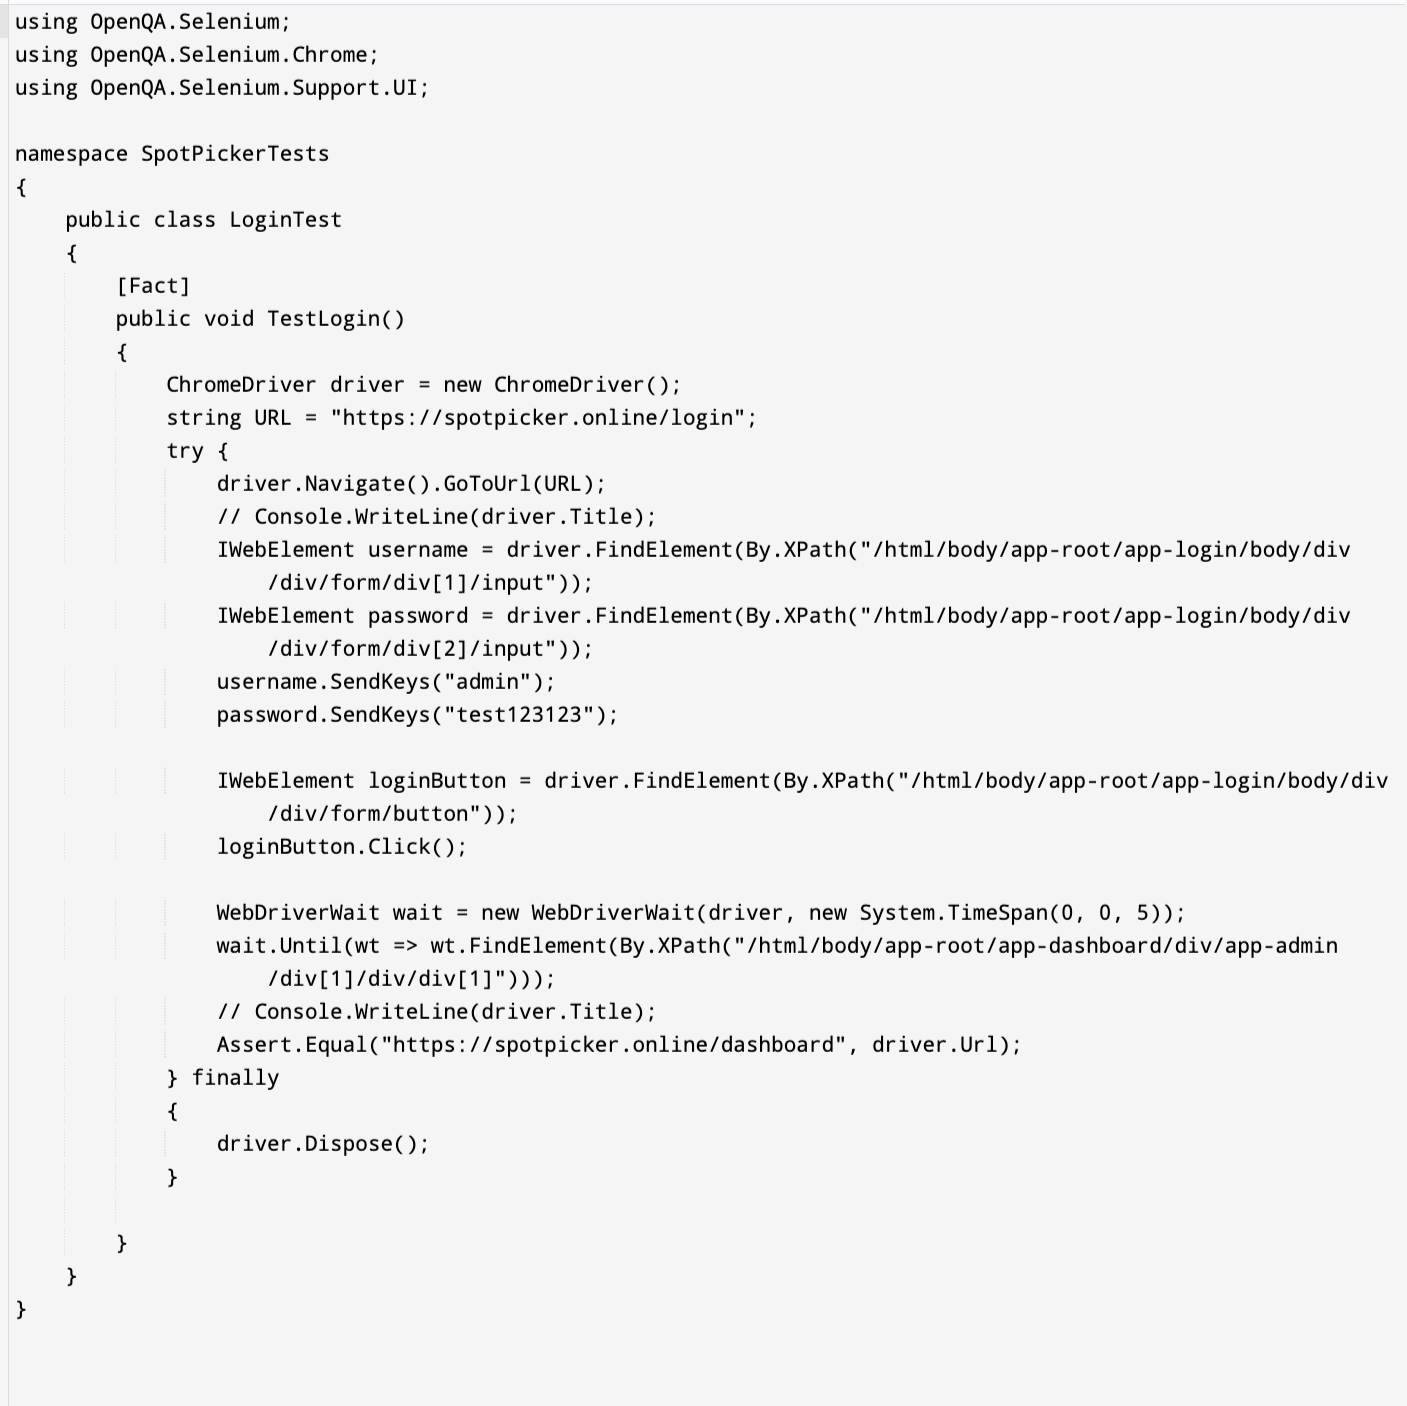
\includegraphics[width=0.7\linewidth]{slike/kod4.png}
			 	\caption{LoginTest}
			 	\label{fig:kod4}
			 \end{figure}
			 
			 
			 \textbf{AdminChangeTest}
			 
			 {Još jedan sistem test, ovaj provjerava funkcionira li promjena nečije uloge od strane admina:}
			 
			 
			 
			 \begin{figure}[hbt!]
			 	\centering
			 	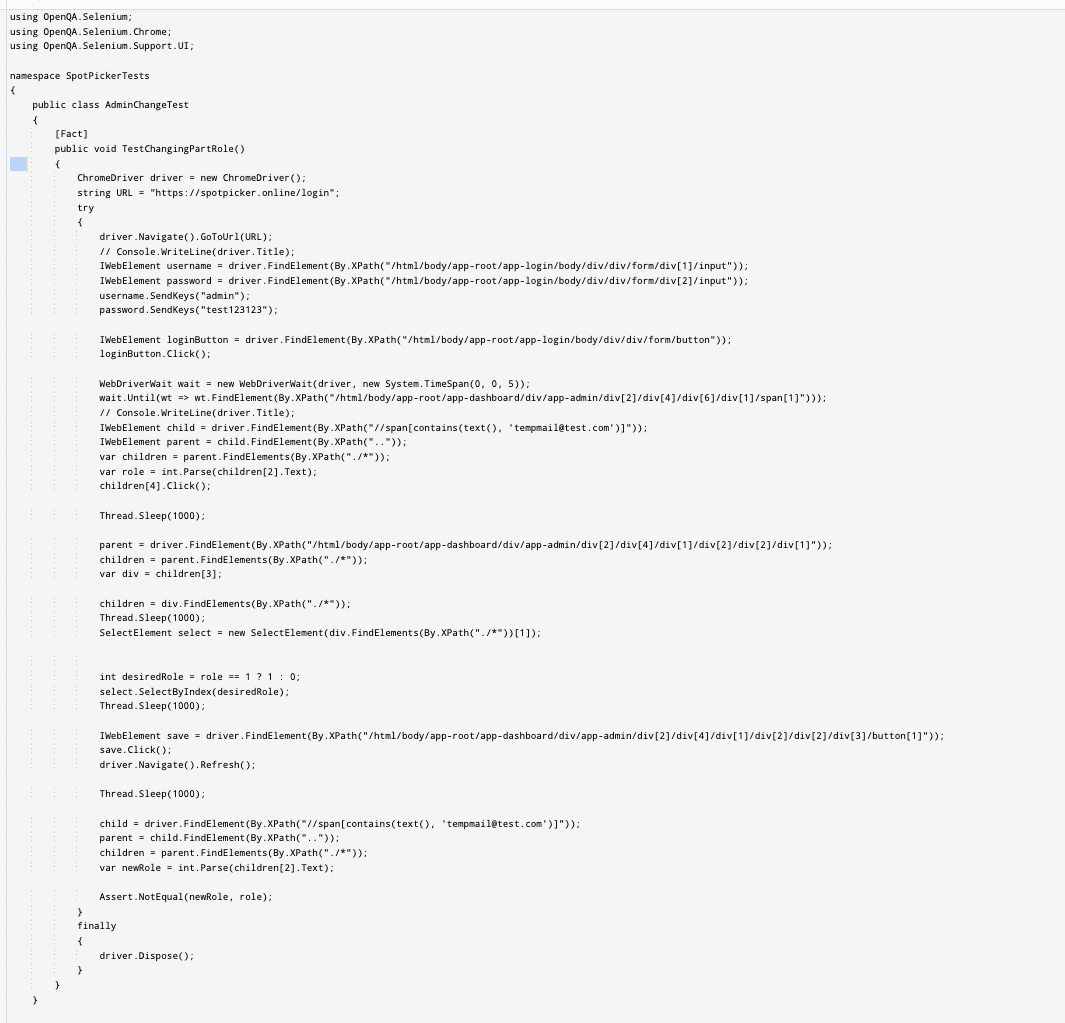
\includegraphics[width=0.7\linewidth]{slike/kod5.png}
			 	\caption{AdminChangeTest}
			 	\label{fig:kod5}
			 \end{figure}
			 
			 
			 
			 
			 {Za pokretanje testova koristili smo xUnit testing framework, ovo je rezultat:}
			 
			 
			 
			 
			 \begin{figure}[hbt!]
			 	\centering
			 	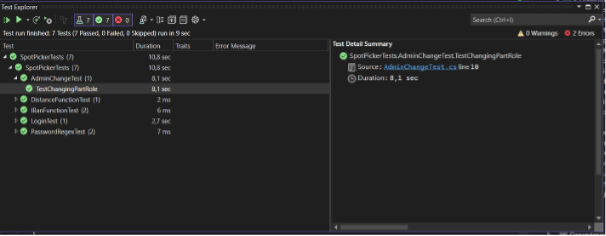
\includegraphics[width=0.7\linewidth]{slike/slikica6.png}
			 	\caption{xUnit testing framework}
			 	\label{fig:slikica6}
			 \end{figure}
			 
			 
			
			\eject 
		
		
		\section{Dijagram razmještaja}
			
			
			
			 {Kako bi se bolje razumjela arhitektura sustava koristi se dijagram razmještaja. On prikazuje arhitekturu programskog sustava tako što pokazuje razmještaj programske potpore i samu topologiju sklopovlja. Svrha dijagrama razmještaja je pružanje pomoći prilikom donošenja raznih odluka u vezi sustava. Poslužiteljsko računalo može obavljati veći broj radnji u isto vrijeme te ga u istom trenutku može koristiti više korisnika. Web poslužitelj te poslužitelj baze podataka nalaze se na poslužiteljskom računalu, a korisnici koriste web poslužitelj za pristup web aplikaciji. Korištena je klijent-poslužitelj arhitektura. Prednosti ove arhitekture je što više klijenata istovremeno može pristupiti poslužitelju te mogu pristupiti funkcionalnostima poslužitelja sa udaljenosti. Komunikacija između računala korisnika, administratora i voditelja parkinga je realizirana putem HTTP veze.}
			 
			 \begin{figure}[hbt!]
			 	\centering
			 	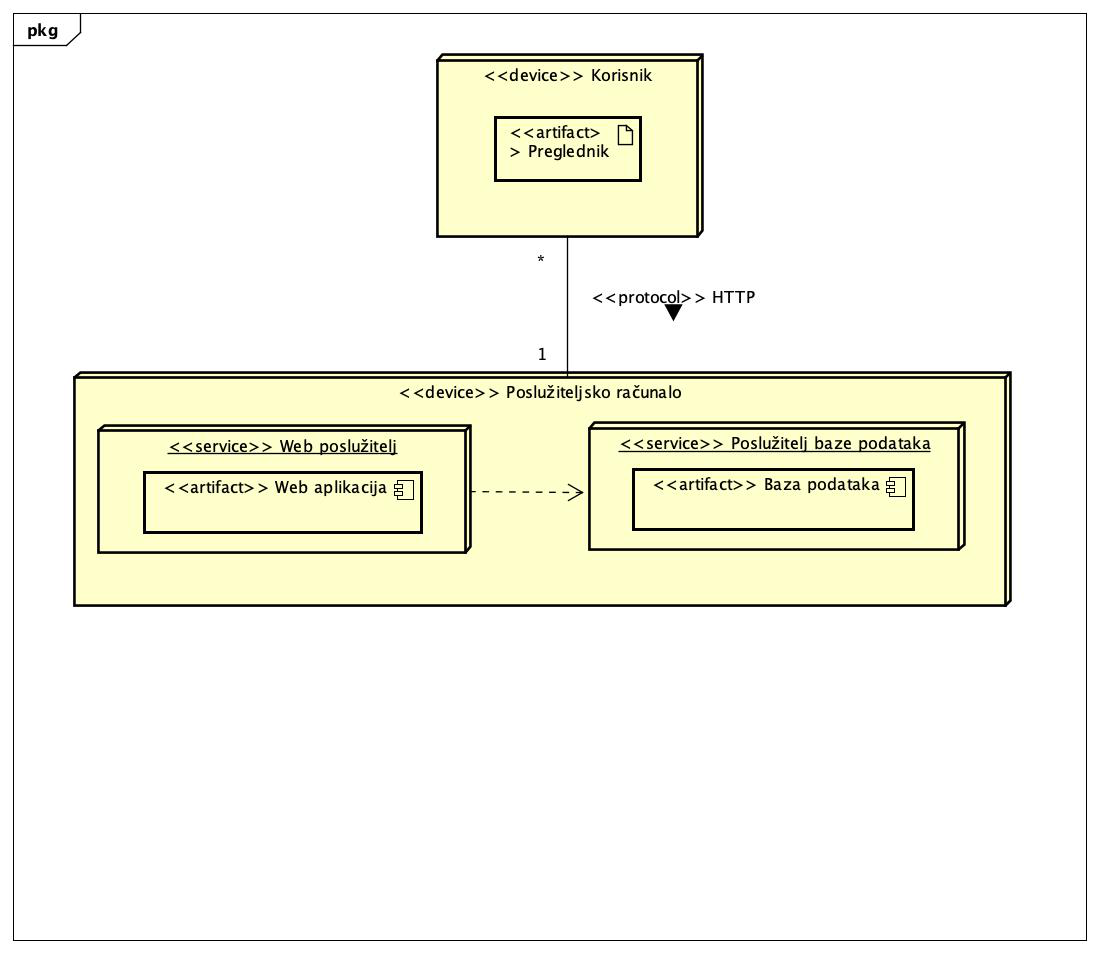
\includegraphics[width=0.7\linewidth]{slike/DijagramRazmjestaja.png}
			 	\caption{Dijagram razmještaja}
			 	\label{fig:DijagramRazmjestaja}
			 \end{figure}
			
			\eject 
		
		\section{Upute za puštanje u pogon}
		
			
		
			 {Postoji server odnosno računalo koje je smješteno u Nizozemskoj i na njemu je instaliran Nginx server koji poslužuje našu aplikaciju. Na tom remote računalu se nalazi frontend, backend i baza podataka. Baza podataka je PostgreSQL i ona je otvorena za konekcije svim IP adresama, potrebna je samo lozinka te se mi spojimo sa svojeg računala na tu bazu koja je u Nizozemskoj i onda ažuriramo nove podatke koje postavljamo. Na taj način bazu podataka ažuriramo i postavljamo, a frontend i backend prvo izgradimo i onda te datoteke pomoću FileZilla, software koji nam olakšava povezivanje sa serverom, pomoću SFTP protokola prebacujemo podatke na remote računalo odnosno naš server. }
			 
			 
			 \begin{figure}[hbt!]
			 	\centering
			 	\includegraphics[width=0.7\linewidth]{slike/datotečnisustav.png}
			 	\caption{prikaz povezivanja u datotečni sustav remote računala}
			 	\label{fig:datotečnisustav}
			 \end{figure}
			 
			 
			 
			 
			 
			 \begin{figure}[h]
			 	\centering
			 	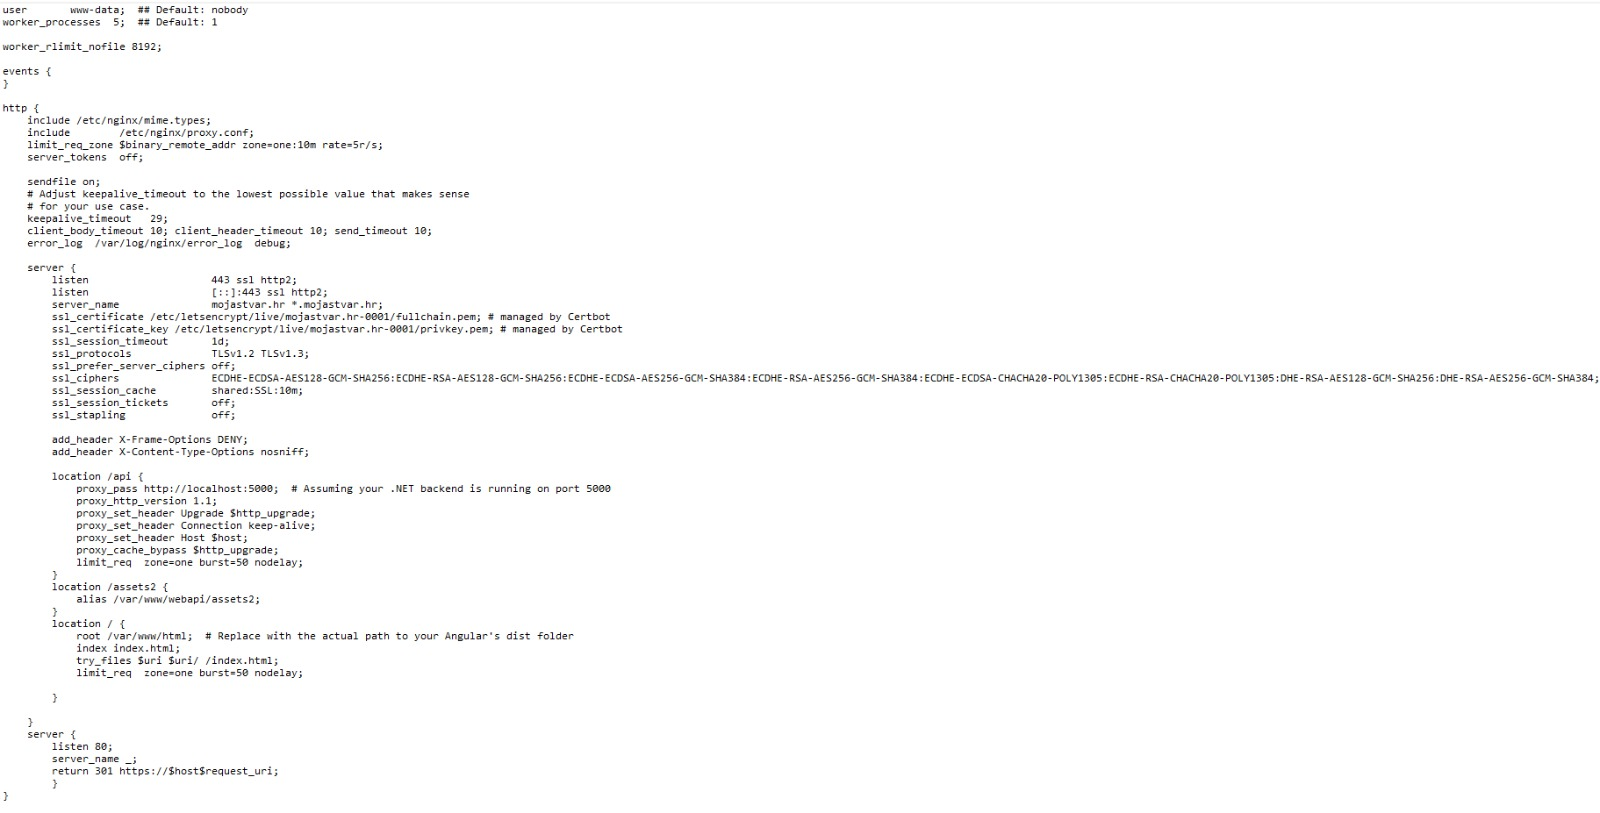
\includegraphics[width=\textwidth,keepaspectratio]{slike/konfiguracijaservera.png}
			 	\caption{prikaz konfiguracije servera}
			 	\label{fig:konfiguracijaservera}
			 \end{figure}
			 
			 
			 
			 \begin{figure}[hbt!]
			 	\centering
			 	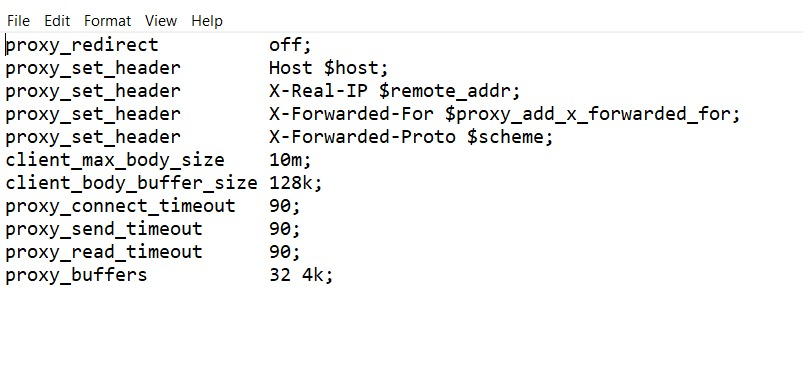
\includegraphics[width=0.7\linewidth]{slike/konfiguracijaproxyja.png}
			 	\caption{prikaz konfiguracije proxyja}
			 	\label{fig:konfiguracijaproxyja}
			 \end{figure}
			 
			 
			 
			 \begin{figure}[hbt!]
			 	\centering
			 	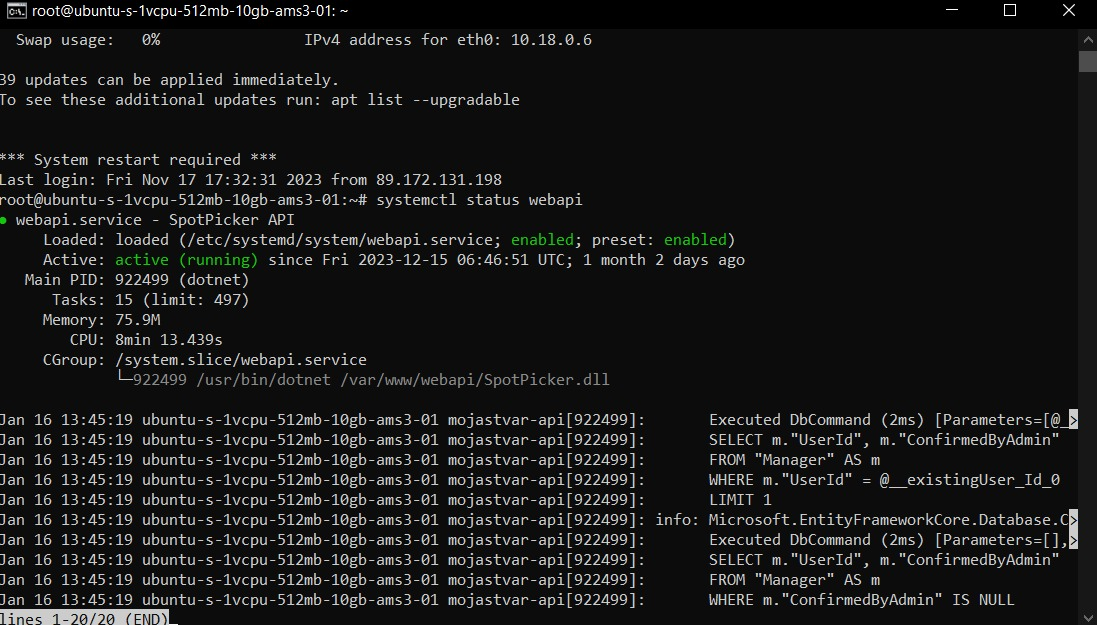
\includegraphics[width=0.7\linewidth]{slike/povezivanjekonzole.png}
			 	\caption{prikaz povezivanja preko konzole na Ubuntu server}
			 	\label{fig:povezivanjekonzole}
			 \end{figure}
			 
			
			
			 
			
			
			\eject 
	\chapter{Zaključak i budući rad}
		
		
		
		 {Zadatak naše grupe bio je razvoj web aplikacije pod nazivom ”SpotPicker”. Ideja  aplikacije je da se korisnicima omoguć rezervacija, naplata parkiranja i pregled slobodnih parkirališnih mjesta za automobile i bicikle. Nakon 12 tjedana timskog rada, ostvarili smo zadani cilj i projekt je zavrsen. Projekt je bio podijeljen u dvije ključne faze, pri čemu je prva faza obuhvatila okupljanje tima, dodjelu projektnog zadatka te temeljito dokumentiranje zahtjeva. Ova faza pokazala se ključnom za uspješnu provedbu projekta, pružajući čvrst temelj za daljnji razvoj sustava.}
		 
		 {Druga faza, iako kraća, zahtijevala je intenzivan rad i samostalnost članova tima. Nedostatak iskustva s određenim alatima i jezicima potaknuo nas je na samostalno učenje kako bismo uspješno ispunili postavljene ciljeve. Dokumentiranje UML dijagrama i izrada popratne dokumentacije bili su ključni za olakšavanje budućeg održavanja i nadogradnje sustava.}
		 
		 {Sudjelovanje u ovom projektu bilo je izuzetno vrijedno iskustvo za sve članove tima. Za većinu nas, ovo je bio prvi ozbiljniji grupni projekt, i moram reći da smo se iznimno dobro snašli. Biti deo tima koji nije imao sukoba, gdje je suradnja bila prirodna, a komunikacija na iznimno zadovoljavajućoj razini, pridonijelo je uspješnosti realizacije projekta.}
		 
		 {Ovaj projekt predstavljao je prvi ozbiljniji susret s tehnologijama kao što su Git i LaTeX za većinu nas. Tijekom procesa razvoja, stekli smo znanje o korištenju modernih radnih okvira u izradi web aplikacija. Iznimno smo zadovoljni postignutim rezultatima i cijelim timskim radom koji je doprinio ostvarenju tih rezultata.}
		 
		 {Ovo iskustvo nas je obogatilo ne samo tehničkim znanjem već i sposobnostima timskog rada i upravljanja projektima. Spremni smo za nove izazove i s veseljem nastavljamo s daljnjim profesionalnim razvojem.}
		  
		 
		   
		   
		
		 
		
		\eject 
	\chapter*{Popis literature}
		\addcontentsline{toc}{chapter}{Popis literature}
	 	
 		
		
		
		\begin{enumerate}
			
			
			\item  Programsko inženjerstvo, FER ZEMRIS, \url{http://www.fer.hr/predmet/proinz}
			
			\item  I. Sommerville, "Software engineering", 8th ed, Addison Wesley, 2007.
			
			\item  T.C.Lethbridge, R.Langaniere, "Object-Oriented Software Engineering", 2nd ed. McGraw-Hill, 2005.
			
			\item  Visual Paradigm, \url{https://online.visual-paradigm.com/}
			
			\item  The Unified Modeling Language, \url{https://www.uml-diagrams.org/}
			
			\item  Astah Community, \url{http://astah.net/editions/uml-new}
		
		\end{enumerate}
		
		 
	
	
	\begingroup
	\renewcommand*\listfigurename{Indeks slika i dijagrama}
	%\renewcommand*\listtablename{Indeks tablica}
	%\let\clearpage\relax
	\listoffigures
	%\vspace{10mm}
	%\listoftables
	\endgroup
	\addcontentsline{toc}{chapter}{Indeks slika i dijagrama}


	
	\eject 
		
	\chapter*{Dodatak: Prikaz aktivnosti grupe}
		\addcontentsline{toc}{chapter}{Dodatak: Prikaz aktivnosti grupe}
		
		\section*{Dnevnik sastajanja}
		
		\textbf{\textit{Kontinuirano osvježavanje}}\\
		
		 \textit{U ovom dijelu potrebno je redovito osvježavati dnevnik sastajanja prema predlošku.}
		
		\begin{packed_enum}
			\item  sastanak
			
			\item[] \begin{packed_item}
				\item Datum: u ovom formatu: \today
				\item Prisustvovali: I.Prezime, I.Prezime
				\item Teme sastanka:
				\begin{packed_item}
					\item  opis prve teme
					\item  opis druge teme
				\end{packed_item}
			\end{packed_item}
			
			\item  sastanak
			\item[] \begin{packed_item}
				\item Datum: u ovom formatu: \today
				\item Prisustvovali: I.Prezime, I.Prezime
				\item Teme sastanka:
				\begin{packed_item}
					\item  opis prve teme
					\item  opis druge teme
				\end{packed_item}
			\end{packed_item}
			
			%
			
		\end{packed_enum}
		
		\eject
		\section*{Tablica aktivnosti}
		
			\textbf{\textit{Kontinuirano osvježavanje}}\\
			
			 \textit{Napomena: Doprinose u aktivnostima treba navesti u satima po članovima grupe po aktivnosti.}

			\begin{longtblr}[
					label=none,
				]{
					vlines,hlines,
					width = \textwidth,
					colspec={X[7, l]X[1, c]X[1, c]X[1, c]X[1, c]X[1, c]X[1, c]X[1, c]}, 
					vline{1} = {1}{text=\clap{}},
					hline{1} = {1}{text=\clap{}},
					rowhead = 1,
				} 
			
				\SetCell[c=1]{c}{} & \SetCell[c=1]{c}{\rotatebox{90}{\textbf{Ime Prezime voditelja}}} & \SetCell[c=1]{c}{\rotatebox{90}{\textbf{Ime Prezime }}} &	\SetCell[c=1]{c}{\rotatebox{90}{\textbf{Ime Prezime }}} & \SetCell[c=1]{c}{\rotatebox{90}{\textbf{Ime Prezime }}} &	\SetCell[c=1]{c}{\rotatebox{90}{\textbf{Ime Prezime }}} & \SetCell[c=1]{c}{\rotatebox{90}{\textbf{Ime Prezime }}} &	\SetCell[c=1]{c}{\rotatebox{90}{\textbf{Ime Prezime }}} \\  
				Upravljanje projektom 		&  &  &  &  &  &  & \\ 
				Opis projektnog zadatka 	&  &  &  &  &  &  & \\ 
				
				Funkcionalni zahtjevi       &  &  &  &  &  &  &  \\ 
				Opis pojedinih obrazaca 	&  &  &  &  &  &  &  \\ 
				Dijagram obrazaca 			&  &  &  &  &  &  &  \\ 
				Sekvencijski dijagrami 		&  &  &  &  &  &  &  \\ 
				Opis ostalih zahtjeva 		&  &  &  &  &  &  &  \\ 

				Arhitektura i dizajn sustava	 &  &  &  &  &  &  &  \\ 
				Baza podataka				&  &  &  &  &  &  &   \\ 
				Dijagram razreda 			&  &  &  &  &  &  &   \\ 
				Dijagram stanja				&  &  &  &  &  &  &  \\ 
				Dijagram aktivnosti 		&  &  &  &  &  &  &  \\ 
				Dijagram komponenti			&  &  &  &  &  &  &  \\ 
				Korištene tehnologije i alati 		&  &  &  &  &  &  &  \\ 
				Ispitivanje programskog rješenja 	&  &  &  &  &  &  &  \\ 
				Dijagram razmještaja			&  &  &  &  &  &  &  \\ 
				Upute za puštanje u pogon 		&  &  &  &  &  &  &  \\  
				Dnevnik sastajanja 			&  &  &  &  &  &  &  \\ 
				Zaključak i budući rad 		&  &  &  &  &  &  &  \\  
				Popis literature 			&  &  &  &  &  &  &  \\  
				&  &  &  &  &  &  &  \\ \hline 
				\textit{Dodatne stavke kako ste podijelili izradu aplikacije} 			&  &  &  &  &  &  &  \\ 
				\textit{npr. izrada početne stranice} 				&  &  &  &  &  &  &  \\  
				\textit{izrada baze podataka} 		 			&  &  &  &  &  &  & \\  
				\textit{spajanje s bazom podataka} 							&  &  &  &  &  &  &  \\ 
				\textit{back end} 							&  &  &  &  &  &  &  \\  
				 							&  &  &  &  &  &  &\\ 
			\end{longtblr}
					
					
		\eject
		\section*{Dijagrami pregleda promjena}
		
		\textbf{\textit{dio 2. revizije}}\\
		
		\textit{Prenijeti dijagram pregleda promjena nad datotekama projekta. Potrebno je na kraju projekta generirane grafove s gitlaba prenijeti u ovo poglavlje dokumentacije. Dijagrami za vlastiti projekt se mogu preuzeti s gitlab.com stranice, u izborniku Repository, pritiskom na stavku Contributors.}
		
	

\end{document} %naredbe i tekst nakon ove naredbe ne ulaze u izgrađen dokument 


